\documentclass{scrreprt}
\usepackage{geometry}
\geometry{a4paper}

\usepackage[english]{babel}
\usepackage[utf8]{inputenc}
\usepackage[parfill]{parskip}
\usepackage{amssymb}
\usepackage{amsmath,mleftright}
\usepackage{euler}
\usepackage{xparse}
\usepackage[toc]{appendix}

\counterwithout{footnote}{chapter}
\usepackage{graphicx}
\graphicspath{ {./images} }

\title{MOBA3 Control System}
\subtitle{
Model Railway Control System\\
System Design Specification and Documentation\\\ \\
Rev. B}
\author{Andreas Wälchli}
\date{\today}

\hyphenation{trans-ceiver}
\hyphenation{trans-ceivers}

\newcommand\n{\char`\\n}
\newcommand\ie{\emph{i.e. }}
\newcommand\eg{\emph{e.g. }}
\newcommand{\code}[1]{\texttt{#1}}


\begin{document}
\maketitle

\tableofcontents

\chapter{Introduction}
The \textsc{Moba3} control system is designed as a replacement for previous control systems.
This upgrade is a complete rework and removes all legacy components from previous versions.
Such a step is obviously not taken without careful consideration.

This document outlines the history of the \textsc{Moba} control systems and presents the rationale behind the move to a completely new system.
It also presents the design goals for the new \textsc{Moba3} system.
Finally it serves as a full specification and documentation of both the hardware and software.

The documentation does not provide detailed information about the software implementation.
It only aims to specify the communications interfaces.
Details about software internals and precise decoder operation are deliberately excluded.

\section{Historical Context}
During the construction of the current model railway the decision was made to use traditional analog control for the trains.
Many models were not yet equipped with digital decoders and a retrofit would have been prohibitively expensive.
Since no industry standard digital solution was used for the train control the decision was made to design and construct a custom digital control solution for all other components of the railway.
This solution would provide a push button based control interface designed as a schematic control board.
This would control all switches, signals and all lighting.

\subsection{MOBA1}
A first design used custom control and decoder boards based on the PIC16F527 microcontroller.
The entire railway was divided into 5 sectors:

\emph{Shadow station}, \emph{left entry to main station}, \emph{right entry to main station}, \emph{track switches} and \emph{lighting}.

Each sector had a \emph{master} board embedded in the control board.
This controlled up to 16 push buttons, 16 LEDs on the control board and continuously transmitted a single 8-bit data packet to the decoders in the railway.
This packet did not encode commands but rather a fixed \emph{desired state}.
Each decoder would receive the current state data and check what modifications to its own outputs had to be done to conform to that state.
As a consequence each decoder required bespoke decoding logic.
The data also had to be encoded very efficiently to fit the fixed-length packet.
The sector \emph{right entry to main station} for example controlled 6 switches, 2 entry signals, 4 exit signals and could drive up to 2 independent paths at once.

Each packet contained a single \emph{even parity bit} and was packed between start and end marker bits:

\begin{table}[ht!]
\centering
\begin{tabular}{ | c | c | c | c | }
\hline
$START$ & $data_{0..7}$ & $parity_0(data)$ & $END$ \\\hline
\end{tabular}
\caption{Packet structure}
\end{table}


Transmission was done over a custom unshielded single-ended single-wire serial data bus with a relatively low baudrate. Every bit of data was transmitted over 3 bus clock cycles.

\begin{table}[ht!]
\centering
\begin{tabular}{ | r | l | }
\hline
encoded bit & transmitted sequence \\\hline\hline
$START$ & \texttt{000} \\\hline
$0$     & \texttt{100} \\\hline
$1$     & \texttt{110} \\\hline
$END$   & \texttt{111} \\\hline
\end{tabular}
\caption{bit encoding}
\end{table}

\subsection{MOBA2}
During the construction and testing of the first system it became clear that this solution was highly limited:
Each sector had its own \emph{master} board and these were not able to exchange any data.
Additionally programs for the PIC16F527 microcontroller needed to be written in MIPS Assembly, which made high-level software design difficult.

It was therefore decided to move the high-level control logic onto a RaspberryPi 3 (RPi) single-board computer.
This allowed for programming of the control logic in high-level languages (Java was used).

The \emph{master} boards for each sector now no longer managed the entire control logic.
They simply transmitted the button states to the RPi and received both the states of the control board LEDs and the sector status packet from the RPi.
Communication between the RPi and the \emph{master} boards was done using SPI in mode $(0,0)$.
The decoders in the railway and the previously described transmission scheme remained in place.

Over time this system also showed its weaknesses:
A model railway is inherently a high-EMI environment.
Relay-based switch drivers and brushed motors, for example, produce significant interference.
But the transmission scheme was not designed with EMI resistance in mind:
An unshielded single-ended serial bus is obviously not suited for such environments.
As a consequence we observed many transmission errors.
To solve this we needed to introduce very extensive error detection.
This slowed the data busses down significantly.
Additional problems manifested themselves as soon as microcontrollers from another production batch were introduced:
The microcontrollers all used internal 4MHz RC oscillators but these had significant variance between batches.
But the bus required relatively tight timings to avoid reception errors.
This could be partially solved by calibrating each decoder controller to the frequency of its \emph{master} board.
But the oscillators would also drift based on the atmospheric climate.
In the end we were forced to introduce a self-calibration routine that would calibrate each microcontroller based on the incoming serial data signal.
This routine would run at every startup and whenever the decoder had too many transmission errors.
The issues of transmission errors could however never be completely solved.

\section{MOBA3}
The issues outlined above eventually lead to the decision to introduce a full redesign before the model railway was completed.
This new solution would be designed with EMI-resistance in mind from the beginning.
It would make away with the sector concept and the state transmissions.
A single controller board would control the entire railway and the decoders would use unified software.

\subsection{Design Goals}
The full redesign of the control system allowed for the definition of clear design goals. These are outlined in the following sections.

\subsubsection{Stability and Standardisation}
The first iterations used a lot of custom concepts and hardware solutions.
For the redesign many of these custom design elements should be replaced with industry standard solutions where applicable.
Where industry solutions are not directly transferrable, they should at least be adapted to our needs.
The design should also try account for the interference issues observed with previous iteration wherever possible.

\subsubsection{Improved Commonality}
The entire system shall use common hardware design as far as feasible:
All boards should use the same microcontroller type and common areas of the PCBs should use identical routing, component and mounting hole positions.
Different decoder types should also share as much hardware as possible.
Care must be taken that this not lead to an overly unified PCB design that tries to cover all possible use cases.
But where external connectivity requirements are shared between multiple decoder types it shall be attempted to use common hardware.
Behavioural distinctiveness should -- where possible -- be provided through software only.

\subsubsection{Ease of Develoment}
The microcontroller type chosen should allow for easy software development in C/C++.
It should also facilitate debugging and prototyping.
Each board should have a clearly defined set of responsibilities as this complicates both development and testing.
E.g. a switch decoder should only be responsible for receive switching commands and for driving the switch motors.

The PCBs should also support in-circuit reprogramming.
Previous iterations required extraction of the microcontrollers for reprogramming.
This made development and testing more tedious and increased the risk for premature wear on the boards and damage to the microcontrollers.

\subsubsection{Scalabilty}
The entire system should be easily scalable through the addition of additional decoders or decoder types.
Where sensible address spaces shall be defined large enough for substantial increase of the number of decoders.
The entire system shall support at least 50\% more decoders per type as is required on introduction.

\chapter{Design Specification}
The \textsc{Moba3} control system consists of a central \emph{controller board} (CTRB), an \emph{I/O interface board} (IIB) and several \emph{decoder boards} (decoder).
The I/O interface board handles button presses, forwards them to the controller board and drives the control panel LEDs based on commands received from the controller board.
The controller board processes button presses and issues corresponding commands to the I/O interface board and the decoders.
The decoders are not as smart as with previous system iterations and do not require bespoke software.
\textsc{Moba3} supports numerous decoder types, each designed for a specific purpose.
At the moment there are decoders for switches, station entry signals, station exit signals and lighting.

\section{Common Hardware}
To facilitate design and scalability we defined a set of common hardware to be used for all board types.
This defines common set of components that should be used if required.
Additional components can be introduced on specific boards if needed.

\subsection{Microcontroller}
Each board uses a single central microcontroller.
The model used is an ATmega328P.
This is the exact same microcontroller as is used on \emph{Arduino Uno} and \emph{Arduino Nano} boards.
This allows for easy prototyping and debugging using that board.
The microcontroller is provided with an external clock signal from a 16Mhz crystal oscillator.
All configuration fuses are set identically to microcontrollers on Arduino boards.
This commonality in configuration between Arduino boards and our \textsc{Moba3} boards also facilitate testing and development.

\subsection{Bus Transceivers}
The data busses (specified below) require RS422/RS485 transceiver chips.
All transceivers should be from the MAX481 transceiver family or compatible hardware.
The MAX481 family consists of multiple different transceivers in different configurations (simplex, half-duplex, full-duplex, etc.).
Any component of this family can be used.
For each board the best suited model can be selected.

\subsection{Multi-Pin Input and Output}
For multi-pin I/O the individual pins should not be connected directly to the microcontroller.
PISO and POSI circuits should be used instead.
Standard ICs used for Arduino-based applications are the CD4021 and 74HC595 ICs for input and output respectively.
These are buffered shift registers that can easily be daisy chained.

The CD4021 is an 8-bit shift register with \emph{parallel load} functionality.
This makes it useful for \emph{parallel-to-serial} data input.

The 74HC595 is an 8-bit shift register with a \emph{tri-state buffered parallel output}.
This makes it useful for \emph{serial-to-parallel} data output.

Both shift registers can be read and written using SPI hardware in mode $(0,0)$.

\section{Data Bus Specification}
The \textsc{Moba3} control system is based on a UART serial bus with a baudrate of 9600.\footnote{higher baudrates up to 2 Mbaud are theoretically possible}
The data is transmitted over differential pairs on an RS422/RS485 derived serial bus.
The differential pairs are driven using MAX481 compatible transceivers operating at 5V.
Physically the data bus uses 8P8C (RJ45) connections for both power (5V only) and data.
There are 2 busses:
The \emph{local bus} and the \emph{remote bus}.
To improve EMI resistance shielded CAT6a cabling\footnote{S/FTP with a grounded shield} is used.
Low power decoders can be powered directly by the bus, higher power decoders do require external power delivery.
Some decoders may require additional voltages.
These should always use external power delivery.
Any externally powered decoder also provides power to the bus.
The current draw on a single connection in the bus is limited to 600mA.
Care must be taken to ensure that no bus segment exceeds this limit.
This can be solved either by introducing additional external power connections where required or by simply connecting decoders strategically -- \eg alternating high-current decoders and low current decoders.

\subsubsection {Bus Loading and Biasing}
In a deviation from the RS422 specification the bus does not need to be terminated. Each decoder loads the differential pair with a $10k\Omega$ resistor. This loading introduces a theoretical limit on the number of supported decoders to around 150. But this is very obviously only a theoretical limit and does not need to be considered further. In case the system should be used for an application with more than around 100 decoders we suggest the introduction active repeaters.

The differential pair is also not biased. The loading resistor equalises the voltage potential in the differential pair on disconnected decoders. The MAX481 transceiver will always read equal voltages as a logical $0$. The transmitters are always powered. For situations where the busses are correctly connected biasing becomes irrelevant as the transmitters will always drive the differential pair.

\subsection{Local Bus Specification}
The \emph{local bus} is a full-duplex bus used for communication between the CTRB and the IOIB that manages I/O on the control panel. 2 differential pairs are used for bidirectional data transmission, the remaining 2 are used for power.

\begin{table}[ht!]
\centering
\begin{tabular}{ |r|l|l|l| }
\hline
pin & colour & function & description \\\hline\hline
  1 & G/     & MOSI\_B  & CTRB transmission, negative channel \\\hline
  2 & G      & MOSI\_A  & CTRB transmission, positive channel \\\hline
  3 & O/     & MISO\_B  & IOIB transmission, negative channel \\\hline
  4 & B      & GND      & ground wire \\\hline
  5 & B/     & GND      & ground wire \\\hline
  6 & O      & MISO\_A  & IOIB board transmission, positive channel \\\hline
  7 & Br/    & VCC      & 5V power \\\hline
  8 & Br     & VCC      & 5V power \\\hline
\end{tabular}
\caption{\emph{local bus} RJ45 pinout}
\end{table}

The \emph{local bus} is a a direct connection bus between the CTRB and the IOIB and must connect exactly one of each of these devices.

\subsection{Remote Bus Specification}
The \emph{remote bus} is a simplex bus used for communication between the CTRB and the decoders. The decoders are connected using daisy chaining. It only carries data from the CTRB to the decoders. The differential pair used for IOIB transmissions on the \emph{local bus} is used for connection sensing on the \emph{remote bus}: Each decoder feeds back power through this pair to the previous board in the chain. This allows for easy identification of a break in the chain. It also ensures that in case a decoder is connected to the \emph{local port} the CTRB is presented with a permanently idle IOIB transmission channel.

\begin{table}[ht!]
\centering
\begin{tabular}{ |r|l|l|l| }
\hline
pin & colour & function & description \\\hline\hline
  1 & G/     & MOSI\_B  & CTRB transmission, negative channel \\\hline
  2 & G      & MOSI\_A  & CTRB transmission, positive channel \\\hline
  3 & O/     & STATUS-  & sensing feedback ground connection \\\hline
  4 & B      & GND      & ground wire \\\hline
  5 & B/     & GND      & ground wire \\\hline
  6 & O      & STATUS+  & sensing feedback 5V \\\hline
  7 & Br/    & VCC      & 5V power \\\hline
  8 & Br     & VCC      & 5V power \\\hline
\end{tabular}
\caption{\emph{remote bus} RJ45 pinout}
\end{table}

Please note that it is not required for the controller transmission channels for the 2 busses are separated. The controller is allowed to transmit all data on both channels. It is however recommended that each channel is driven by a separate transceiver. The decoders can simply pass through the differential pair and use stub connections to their local receivers. If required it is also possible to add repeating transceivers to the chain. This should however not be necessary as the specified design should tolerate distances of more than 100m.

\section{Data Transmission Format}
Unlike the previous systems \textsc{Moba3} transmits \emph{commands}, not \emph{states}. All commands follow a common structure, but each decoder type defines its own \emph{payload semantics}. It is however generally required that all commands are human readable and restricted to the printable ASCII character set.
Each command is transmitted as a \emph{line} terminated by a line break (\texttt{\n}) character.

There are 3 line formats:
\emph{display command} and \emph{decoder command} lines are transmitted by the CTRB.
\emph{button event} lines are transmitted by the IOIB.

\subsection{Binary Encoding and Endianness}
Since we are restricted to the printable ASCII character set we need to use an alphanumeric encoding for binary data.
A hexadecimal encoding is used, where for each byte the high nibble is transmitted before the log nibble.
For example, the number $0x2f$ would be transmitted as the sequence \texttt{2f}.
Hexadecimal values are always transmitted in lowercase letters.

Multi-byte values also use a hexadecimal encoding.
The bytes are ordered in \emph{big-endian}:
The least significant byte is transmitted first and the most significant byte is transmitted last.
For example, the 16-bit number $0xba42$ is transmitted as the sequence \texttt{42ba}.
This holds true for values of any size.

\subsection{Display Command}
Display commands begin with a constant character prefix \texttt{D}.
This is followed by a 12 character hexadecimal encoding of the 48-bit display data.
Each bit of the display data directly corresponds to a single LED on the control board.
The display data ($data$) is treated as a single 6 bytes long unsigned integer.

\begin{table}[ht!]
\centering
\begin{tabular}{ |l|l|l| } 
\multicolumn{1}{l}{$0$} & \multicolumn{1}{l}{$1..$} & \multicolumn{1}{l}{$13$} \\ \hline
\texttt{D} & $HEX(data)$ & \texttt{\n} \\\hline
\end{tabular}
\caption{display command structure}
\end{table}

Example: \texttt{D012436fdea12\n}\\
Regex: \texttt{D[0-9a-f]\{12\}\n}

\subsection{Decoder Command}
Decoder commands start with a \emph{type selector} ($type$) and a \emph{decoder address} ($addr$).
After this common prefix a decoder specific payload of arbitrary length ($pld$) can follow.
The command is terminated -- as always -- with a line break.
While theoretically arbitrary, the payload length should not exceed 12 characters.

\begin{table}[h!]
\centering
\begin{tabular}{ |l|l|l|l| } 
\multicolumn{1}{l}{$0$} & \multicolumn{1}{l}{$1$} & \multicolumn{1}{l}{$2..\#pld+2$} & \multicolumn{1}{l}{$\#pld+3$} \\ \hline
$type$ & $HEX(addr)_0$ & $pld$ & \texttt{\n} \\\hline
\end{tabular}
\caption{decoder command structure}
\end{table}

\subsubsection{Type Selector}
The type selector indicates the decoder type the command is relevant for.
Each decoder type has a unique type selector associated with it.
Type selectors are always capital letters.

\begin{table}[ht!]
\centering
\begin{tabular}{ |l|l| }
\hline
$type$ & decoder type \\\hline\hline
\texttt{A} & station exit signals \\\hline
\texttt{D} & \emph{reserved: used for display commands} \\\hline
\texttt{E} & station entry signals \\\hline
\texttt{L} & lighting \\\hline
\texttt{W} & railway switches \\\hline
\end{tabular}
\caption{assigned type selectors}
\end{table}

\subsubsection{Decoder Address}
The second byte encodes the decoder address.
The address is a hex-encoded 4-bit number.
This is a special case where hexadecimal numbers do not use an even number of characters.
At the moment all addresses must lie in the range $1..9$, but it is possible to relax this to the entire $0..f$ range in a future revision.
In addition to a specific address there is also a \emph{broadcast address} that is accepted by all decoders of a specific type.
This address is the character "\texttt{+}".

\subsubsection{Command Payload}
The payload $pld$ is an arbitrary character sequence with a minimum length of 1 and a maximum length of 12.
The payload must match the regular expression \texttt{[a-z0-9!]\{1,12\}}.
This limitation is primarily introduced to ensure that no command payload contains uppercase letters.
These could be incorrectly interpreted by a decoder as the start of a command line.
The list of allowed characters may be expanded in future revisions.

Regex: \texttt{[AELW][0-9+][a-z0-9!]\{1,12\}\n}

\subsection{Button Event}
The IOIB continuously monitors the states of all push buttons on the control panel.
Whenever a change in a button state is detected, a corresponding \emph{button event} is sent from the IOIB to the CTRB.

Each button has a 1 byte \emph{button address} ($addr$).
As the third character, a \emph{direction identifier} ($dir$) is sent.
When a new button is pressed, a \emph{key-down} event is sent, when a button is released, a \emph{key-up} event is sent.

\begin{table}[h!]
\centering
\begin{tabular}{ |l|l|l| } 
\multicolumn{1}{l}{$0..1$} & \multicolumn{1}{l}{$2$} & \multicolumn{1}{l}{$3$} \\ \hline
$HEX(addr)$ & $dir$ & \texttt{\n} \\\hline
\end{tabular}
\caption{button event data structure}
\end{table}
\begin{table}[h!]
\centering
\begin{tabular}{ |l|l| } 
\hline
event type     & $dir$ \\\hline\hline
\emph{key-down} event & \texttt{+} \\\hline
\emph{key-up} event   & \texttt{-} \\\hline
\end{tabular}
\caption{button event direction identifiers}
\end{table}

Examples: \texttt{23+\n}, \texttt{1a-\n} \\
Regex: \texttt{[1-4][0-9a-f][+-]\n}


\chapter{Hardware Support}
\section{Switches}
\textsc{Moba3} supports magnetic switch motors including \emph{Märklin} articles 74491 and 75491 and \emph{ROCO} article 10030. Older \emph{Märklin} K switches with integrated motors are also supported.

\textsc{Moba3} limits the active time for all motors.
Therefore there is no need for limit switches in any switch motors.
They can be used but if there are issues with the driving power it is recommended to disable limit switches in the switch motors.

\section{Signals}
\textsc{Moba3} supports swiss type L home signals and distance signals with up to 4 lights.
The lights for the home signals are labelled top-down as $G$, $R$, $O$ and $G'$.
The lights for the distance signals are labelled clockwise starting in the top left corner as $o'$, $o''$, $g'$ and $g''$.
The supported signal aspects are the following:\footnote{FDV R300.2 A2020 d -- sections 5.2.2 - 5.2.7}

\begin{table}[ht!]
\centering
\begin{tabular}{ |c|c|c|c| }
\hline
\textbf{0}/\textbf{0*} & \textbf{1}/\textbf{1*} & \textbf{2}/\textbf{2*} & \textbf{3}/\textbf{3*} \\\hline
stop & full speed & 40km/h & 60km/h \\\hline 
 & & & \\

\includegraphics[width=20px]{signal/0} &

\includegraphics[width=20px]{signal/1} &

\includegraphics[width=20px]{signal/2} &

\includegraphics[width=20px]{signal/3} \\

\includegraphics[width=40px]{signal/0s} &

\includegraphics[width=40px]{signal/1s} &

\includegraphics[width=40px]{signal/2s} &
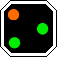
\includegraphics[width=40px]{signal/3s} \\\hline

$R$ & $G$ & $G,O$ & $G,G'$ \\
$o',o''$ & $g',g''$ & $ o',g'$ & $o',g',g''$ \\\hline

\end{tabular}
\caption{supported type L signal aspects}
\end{table}

\section{Lighting}
\textsc{Moba3} does not place any restrictions on the type of lighting that can be used:
The light decoders provide simple digital outputs.
These do not carry a lot of power and should not be used to power lighting elements directly.

The recommended way to power external lighting is to use an NMOS transistor that switches the load to ground.

\begin{figure}[h!]
    \centering
    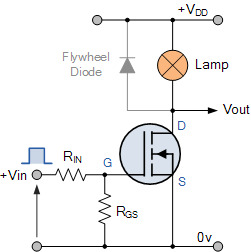
\includegraphics[width=0.5\textwidth]{transistor-tran21}
    \caption{example driving circuit for lighting}
    \label{fig:ctrb}
\end{figure}

\chapter{Circuit Boards}
At the moment there are 4 board designs in use:
The \emph{controller board} (CTRB), the \emph{I/O Interface Board} (IOIB), a \emph{general purpose decoder board} and the \emph{switch decoder board}.
The general purpose decoder board is used for all signal decoders and for light decoders.
All boards have many similarities in component selection, circuitry and routing.

All boards use a 3 pin power connector.
Usually only pins 1 and 2 are used for ground and 5V respectively.
Pin 3 can be used to provide an additional voltage to the board.

\section{Controller Board}
\begin{figure}[h!]
    \centering
    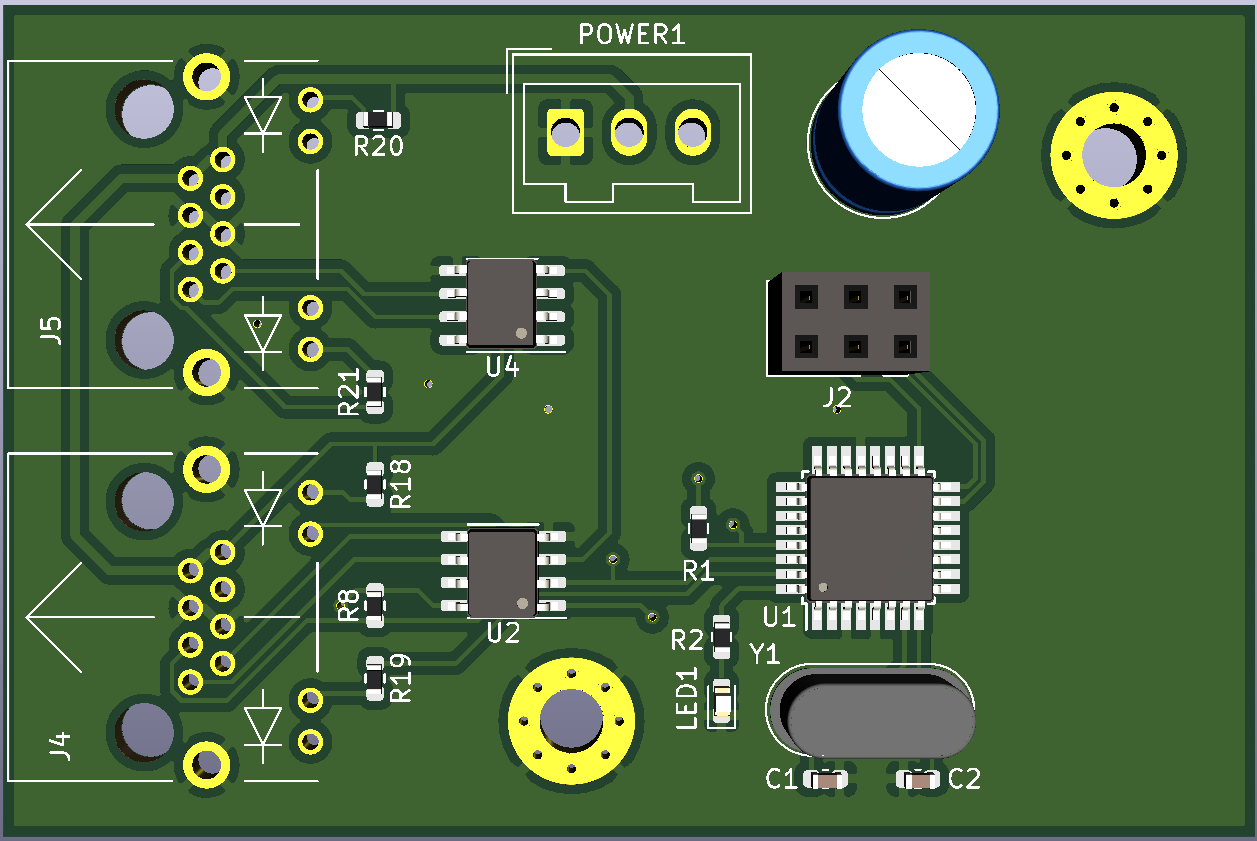
\includegraphics[width=0.6\textwidth]{controller}
    \caption{controller board (CTRB)}
    \label{fig:ctrb}
\end{figure}

The \emph{controller board} (CTRB) is the simplest of the PCB designs currently in use.
It only contains a power connector (\texttt{POWER1}), a microcontroller with the associated circuitry and 2 RJ45 connectors with their corresponding transceiver chips.
\texttt{J2} is a mirrored AVR-ICP-6\footnote{in-circuit programming connector used for AVR microprocessors} connector:
The pinout nearly matches a standard AVR-ICP-6 interface, but the top and bottom rows are swapped.

Each RJ45 connector is used for one of the two busses:
\texttt{J4} provides a connection to the \emph{local bus}.
\texttt{J5} is used for the \emph{remote bus}.
It is recommended that this board is always externally powered to provide a power injection point for both busses.

\section{I/O Interface Board}
\begin{figure}[h!]
    \centering
    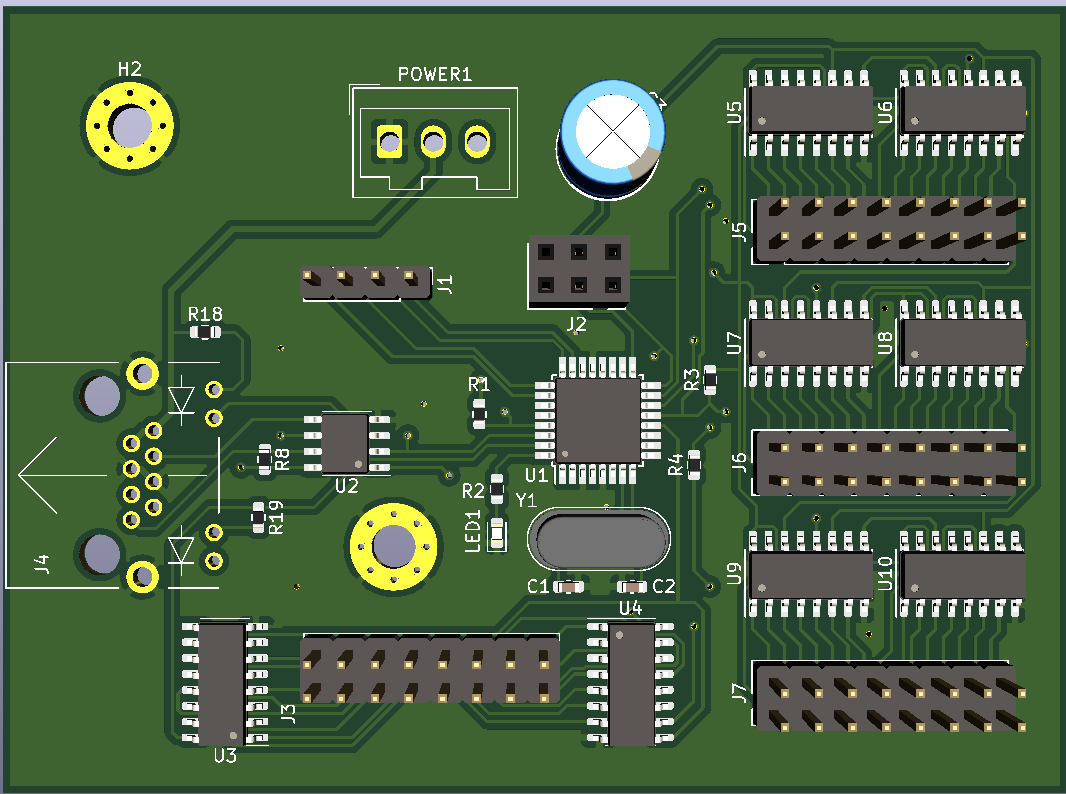
\includegraphics[width=0.8\textwidth]{interface}
    \caption{I/O interface board (IOIB)}
\end{figure}

The \emph{I/O interface board} (IOIB) monitors the push-buttons and drives the LEDs of the control panel.

The \texttt{POWER1} and \texttt{J2} connector are identical to those on the CTRB.
The singular RJ45 connector \texttt{J4} connects to the \emph{local bus}.
The remaining connectors handle \emph{input} and \emph{output}.

\subsection{Input Connectors}
The control panel buttons are divided into 4 sectors of up to 16 buttons each.
The IOIB regularly scans all 4 sectors individually.

The buttons need to be wired in a very specific way:
Each sector has a common \emph{feed pin}.
One terminal of all buttons in one sector needs to be tied to this \emph{feed pin}.
The second terminal is connected to one of the 16 \emph{sense pins} through a series diode.
This diode needs to be oriented with the anode connected to the button and the cathode to the sense pin.
This arrangement leads to a button matrix where for every combination of feed pin sense pin there is exactly one button between these two.
That way when powering the feed pin of one sector the sense pins of all currently pressed buttons of that sector are powered.

The 4-pin connector \texttt{J1} exposes the 4 feed pins for the 4 sectors.
The 16-pin connector \texttt{J3} exposes the 16 sense pins.
All pins of \texttt{J3} require an external pull-down resistor:
The sense pins do posses some stray capacitance.
Due to the diode arrangement residual charges may not dissipate sufficiently quickly through leakage currents alone.
A relatively high resistance\footnote{about $10k\Omega$ should work fine} should be used to not overload the button diodes.

The figure below shows a possible wiring solution.
The horizontal rows \texttt{1} and \texttt{2} are \emph{feed pins}.
The vertical rows \texttt{A} and \texttt{B} are \emph{sense pins}.
It is irrelevant on which side of the button the diode is attached as long as it retains its orientation.

\begin{figure}[h!]
    \centering
    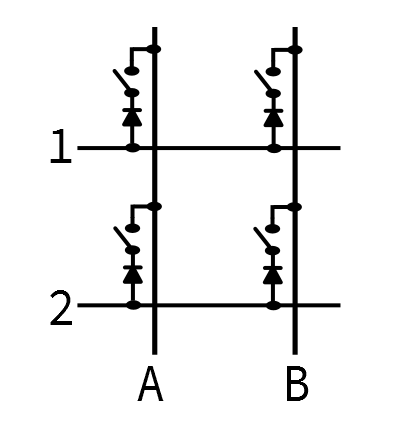
\includegraphics[width=0.4\textwidth]{button-matrix}
    \caption{button matrix schemtic}
    \label{fig:ctrb}
\end{figure}

\subsubsection{Button Addressing}
The following simple formula provides a simple way to calculate the button address from a combination of a feed pin and a sense pin:
\[addr = 16 * (feed - 1) + sense - 1\]

Example:
Button 4 of sector 2 would have the button id $0x13$.\footnote{pin numbers are 1-indexed}

\subsection{Output Connectors}
The remaining connectors (\texttt{J5}, \texttt{J6} and \texttt{J7}) handle \emph{output} - \ie the control panel LEDs.
Each connector provides signals for 16 LEDs.
These pins are directly connected to the 74HC595 shift registers.
While low-power devices could be directly connected to these digital pins it is recommended to use these pins only to drive the gates on external NMOS transistors.
In that configuration the NMOS does not require a pull-down resistor on the gate pin as the IOIB pins are always actively driven.

The 3 connectors are arranged in software as 6 bytes of data.
\texttt{J5} exposes the 2 least significant bytes while \texttt{J7} exposes the 2 most significant bytes.
On each connector pin 1 is the least significant bit of the less significant byte.
\begin{table}[h!]
\centering
\begin{tabular}{ |c|c|c|c|c|c| } \hline
\multicolumn{2}{ |c| }{\texttt{J5}} & \multicolumn{2}{ |c| }{\texttt{J6}} & \multicolumn{2}{ |c| }{\texttt{J7}} \\\hline
pins 1-8 & pins 9-16 & pins 1-8 & pins 9-16 & pins 1-8 & pins 9-16  \\\hline\hline
$data_0$ & $data_1$  & $data_2$  & $data_3$  & $data_4$  & $data_5$ \\\hline
\end{tabular}
\caption{output pin assignments}
\end{table}

%\pagebreak
\section{Decoder Boards}
The decoder boards share much of the basic hardware.
Specifically the power connector, the programming header and the 2 RJ45 connectors are all arranged identically on all decoders.
Also the microprocessor and all basic support components share common placement and trace routing.

\begin{figure}[h!]
    \centering
    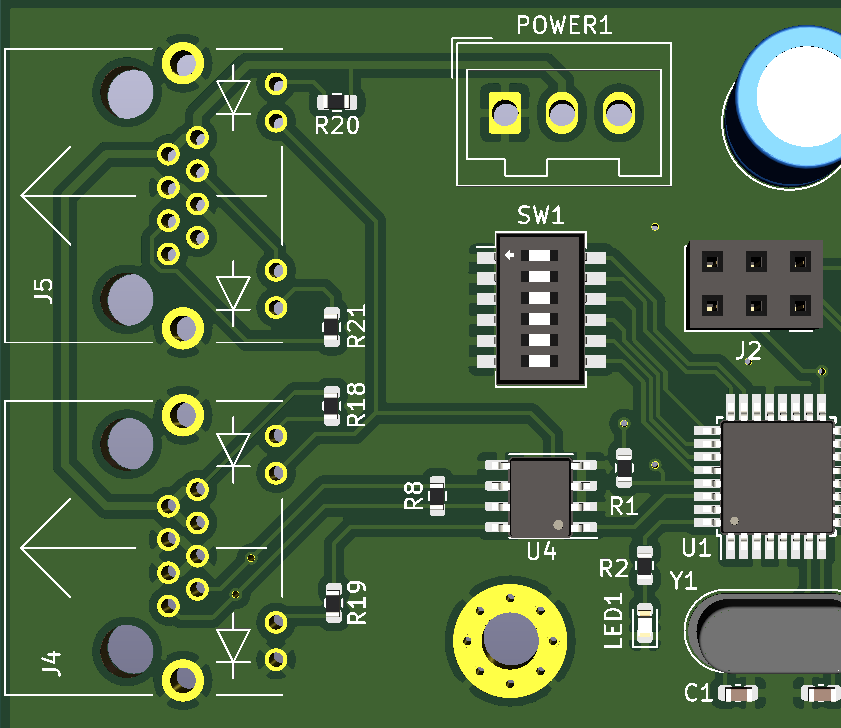
\includegraphics[width=0.4\textwidth]{decoder_general}
    \caption{common area of decoder PCBs}
\end{figure}

On the decoder boards the 2 RJ45 connectors are used for daisy chaining the \emph{remote} bus.
The connector \texttt{J4} is used as the \emph{input} -- \ie the connection to the CTRB or a \emph{previous} board.
The second connector -- \texttt{J5} -- is the \emph{output}.
This connector is used to connect to the \emph{next} board in the chain.
At the last board in the chain this connector can simply be left disconnected and no bus termination is required.

The power connector (\texttt{POWER1}) can be used to externally power the decoder and to provide power to the bus.
On low-power boards it can be left unpopulated or disconnected.

The 6-channel DIP-switch \texttt{SW1} can be used to provide configuration data to the microprocessor.
This could -- for example -- be used to configure the decoder type and address.
The header is provided on all decoders but is not required to be populated if not needed by a decoder.

Please note that the mounting holes are plated and the plating is connected to the ground plane of the board.
To ensure balanced currents on the bus power wires it is recommended to ensure that the mounting screws -- and thereby the mounting holes -- remain electrically isolated from any external ground connection on boards that are bus powered.
On externally powered boards this isolation is not required.

%\pagebreak
\subsection{General Purpose Decoder}
\begin{figure}[h!]
    \centering
    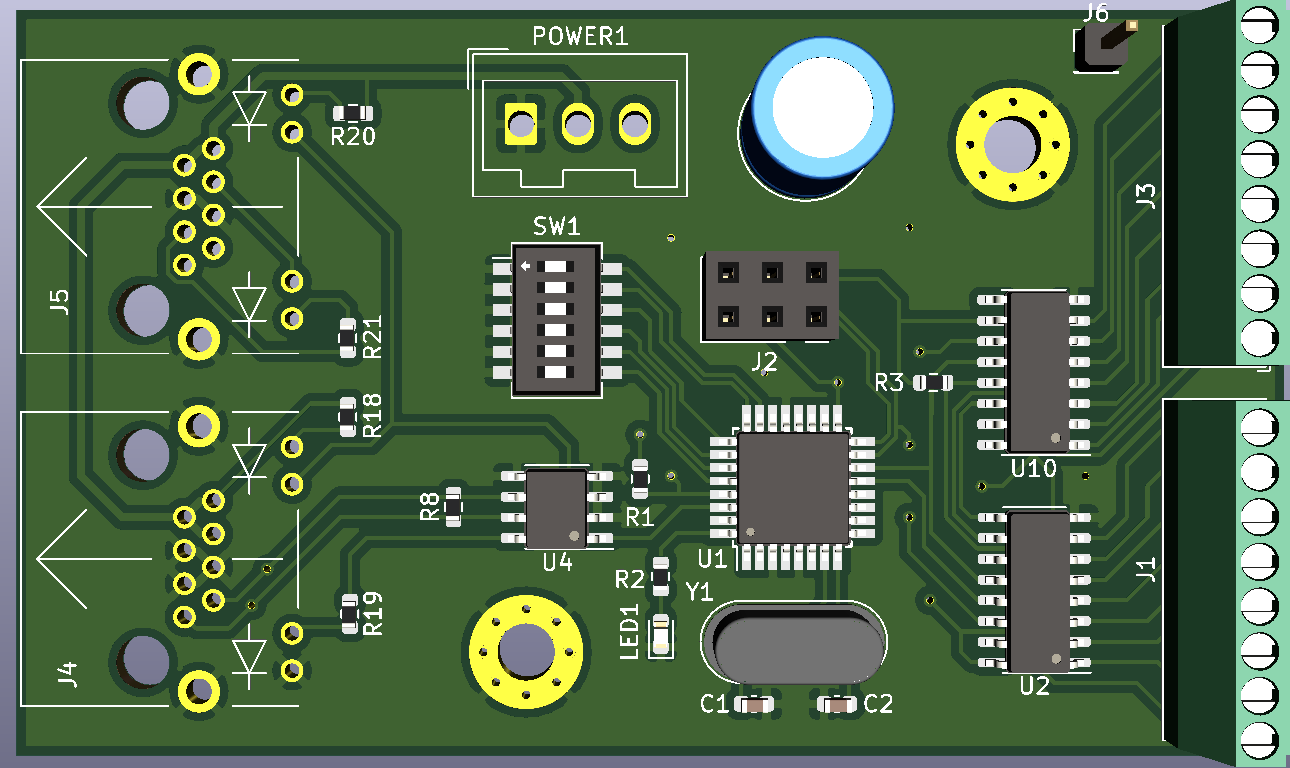
\includegraphics[width=0.6\textwidth]{common_decoder}
    \caption{general purpose decoder board}
\end{figure}

Many functions of the control system require simple digital -- or low-power -- pins.
The \emph{general purpose decoder} provides a generic hardware platform for all these uses.
It is the simplest of the decoder boards and is used for all signal decoders and for lighting.
This board exposes up to 16 pins that are directly wired to the parallel output of two 74HC595 shift registers.
The pins do have tri-state support.
This feature can of course be controlled by the individual decoder software.

The connectors \texttt{J1} and \texttt{J3} expose the 16 output pins.
\texttt{J1} holds the first 8 pins, \texttt{J3} the rest.
In a situation where less than 9 pins are used the header \texttt{J3} and 
the shift register \texttt{U10} can remain unpopulated.
When using the output pins to directly power external components it must be ensured that each pin does not exceed the maximum pin current and each connector does not exceed the maximum port current for the specific shift register used.
Power usage should probably be kept below $10mA$ per pin.

In some situation the output pins may be used as open collectors to power low power devices (\eg LEDs).
These do require a power supply.
If the board is bus-powered the power supply to the external devices should also be taken from the board to keep the currents through the power cables on the bus balanced.
The power may either be taken from the \texttt{POWER1} connector or from the auxiliary pin \texttt{J6} which is also connected to the 5V rail of the board.

%\pagebreak
\subsection{Switch Decoder}
\begin{figure}[h!]
    \centering
    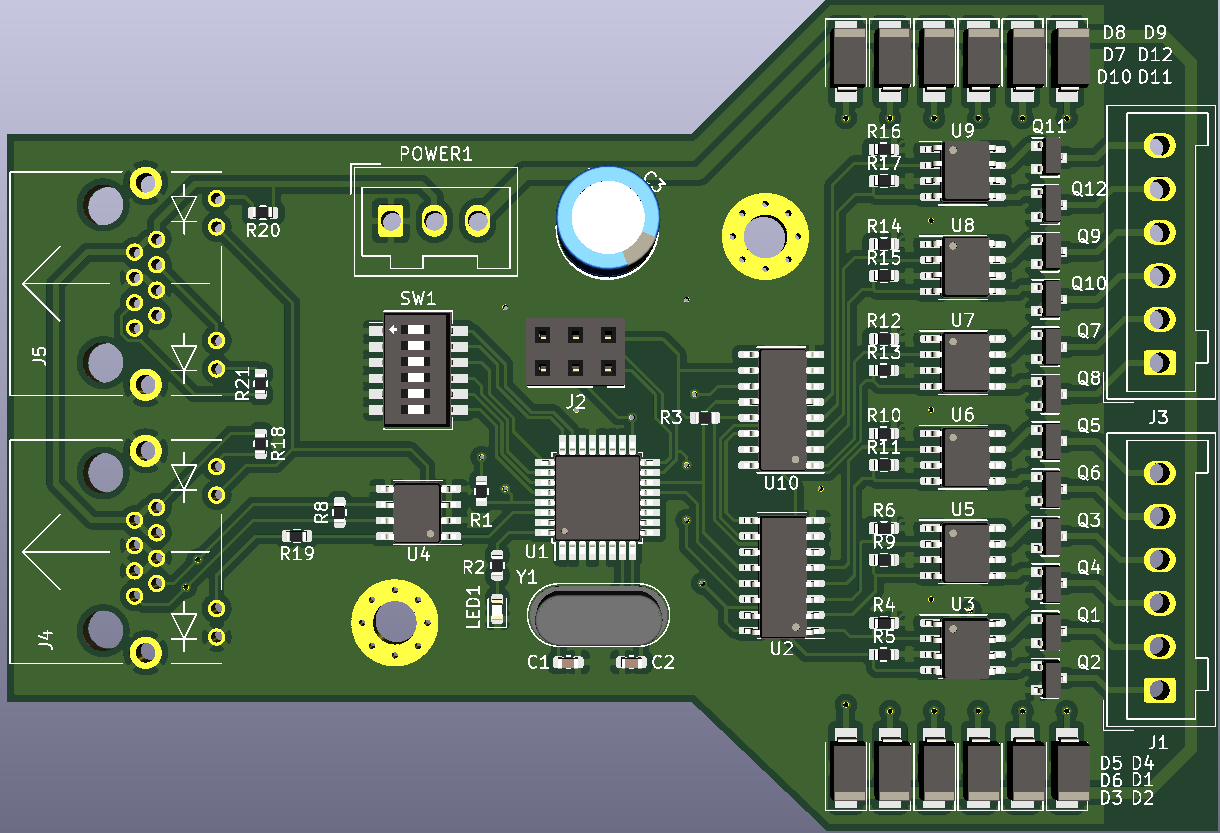
\includegraphics[width=0.7\textwidth]{switch_decoder}
    \caption{switch decoder board}
\end{figure}

Currently the only decoder type with bespoke hardware is the switch decoder.
Each switch decoder allows control of up to 6 switches.

\texttt{J1} and \texttt{J3} provide open collector connections for 3 switches each.
The first pin of each switch should always be connected to the motor pole that pulls the switch into the \emph{straight-through} position.

Each pin is switched to ground through an NMOS transistor with a MOSFET driver IC to minimise switching times.
In addition each pin is also connected to a flyback diode.
Switch motors are usually inductive loads and when switching of a motor pole a voltage spike may occur that could be destructive to the switching transistor.
The on-board high-current schottky diodes protect the transistors from any such voltage spikes.

A connection to the power supply voltage of the switches is required for the flyback diodes to work properly.
The generally unused third pin of the power connector (\texttt{POWER1}) is connected to the cathode of all flyback diodes.
It should be connected to the 24V power rail powering the switches.
Failure to connect the 24V rail could lead to destructive failure of the NMOS transistors due to the drain-source voltage exceeding its limit.
For this reason it is recommended to verify a stable connection upon installation.
A voltage measurement between the cathode of any flyback diode and an exposed mounting hole plating can be used for this purpose.

\chapter{Decoder Type Specifications}
Each decoder type has its own behaviour and command structure.
The decoder command structures in essence define an \emph{instruction set} of instructions sent from the CTRB to the decoders to control the model railway.
The following sections provide detailed specifications for all currently supported decoder types and their individual commands.

\section{Switch Decoder}
Each switch decoder controls up to 6 switches at once.
The switches have a limited drive time (2000ms) after which the switch motor is disabled.
The switching time limits are handled for each switch individually.
While the relatively long switching time should allow switches to fully transition during a switching action.

It is possible that simultaneous switching actions drop the supply voltage.
To avoid this issue it is recommended to send switch commands sequentially over some time.
That way each switch can profit from the full power of the power supply capacitors and between the switching actions the power supply can recover.

\subsection{Pinout}
\begin{table}[ht!]
\centering
\begin{tabular} { |c|c|c|c|c|c||c|c|c|c|c|c| }

\hline
\multicolumn{6}{ |c|| }{\texttt{J1}} &
\multicolumn{6}{ |c|  }{\texttt{J3}} \\\hline

1 & 2 & 3 & 4 & 5 & 6 &
1 & 2 & 3 & 4 & 5 & 6 \\\hline\hline

a & b &
a & b &
a & b &
a & b &
a & b &
a & b \\\hline

\multicolumn{2}{ |c|  }{Sw 1} &
\multicolumn{2}{ |c|  }{Sw 2} &
\multicolumn{2}{ |c|| }{Sw 3} &
\multicolumn{2}{ |c|  }{Sw 4} &
\multicolumn{2}{ |c|  }{Sw 5} &
\multicolumn{2}{ |c|  }{Sw 6} \\\hline


\end{tabular}
\caption{switch decoder pinout}
\end{table}


\subsection{Command Structure}
The switch decoders can receive commands for any number of switches at once.

\begin{table}[ht!]
\centering
\begin{tabular}{ |c|c||c|c||c| } 
\multicolumn{1}{l}{$0$} & \multicolumn{1}{l}{$1$} & \multicolumn{1}{l}{$2i$} & \multicolumn{1}{l}{$2i+1$} & \multicolumn{1}{c}{2n+2} \\ \hline
\texttt{W} & $addr$ & $sid_i$ & $cmd_i$ & \texttt{\n} \\\hline
\end{tabular}
\caption{switch command structure}
\end{table}

Each $(sid_i,cmd_i)$ pair is treated as a single command for one switch.
$sid_i$ is the switch id (\texttt{1}-\texttt{6}) for which $cmd_i$ should be executed.
It is not allowed to send two commands for one switch within a single packet.
If multiple commands are sent for a single switch the decoder behaviour is not defined.
Currently there are 3 supported commands:

\begin{table}[ht!]
\centering
\begin{tabular}{ |l|l| }
\hline
$cmd_i$ & command \\\hline\hline
\texttt{a} & move switch to \emph{straight} track \\\hline
\texttt{b} & move switch to \emph{diverging} track \\\hline
\texttt{!} & reapply previous command \\\hline
\end{tabular}
\caption{supported switch commands}
\end{table}

Switches are moved by the commands \texttt{a} and \texttt{b}.
Generally a decoder will drive a switch motor if it believes a switch to already be in the desired position
-- \ie repeated commands are ignored.
There are however situations where a switch is in a different position than the decoder has driven it to:
A switch could have been moved manually or the switch power supply may have been unpowered when the decoder last drove the switch motor.
For these situations the command \texttt{!} was introduced. It repeates the previous command for the switch.

Example: \texttt{W21a2b3!4a5b6!\n} \\
Regex: \texttt{W[1-9+]([1-6][ab!])\{1,6\}\n}

\section{Exit Signal Decoder}
Each exit signal decoder can control up to 4 exit signals with up to 4 signal LEDs each.
While full 4-LED signals are supported signals with reduced capabilities can also be connected and the pins for unsupported LEDs can simply remain disconnected.
Such a "degraded" signal would simply be incapable of showing some aspects -- \eg a 3-LED signal without $G'$ would be incapable of displaying aspect \textbf{3} and would simply show aspect \textbf{1} instead.
A signal with only 2 LEDs -- $G$ and $R$ -- would only be able to show aspects \textbf{0} and \textbf{1}.
Any other aspects would be displayed as aspect \textbf{1}.

The power-on idle state for all signals is aspect \textbf{0}.

\begin{table}[ht!]
\centering
\begin{tabular} { |c||c|c|c|c| }
\hline
& \multicolumn{4}{|c|}{signal aspect} \\\hline
signal type & \textbf{0} & \textbf{1} & \textbf{2} & \textbf{3} \\\hline\hline
2 LEDs & $X$ & $X$ &     &     \\\hline
3 LEDs & $X$ & $X$ & $X$ &     \\\hline
4 LEDs & $X$ & $X$ & $X$ & $X$ \\\hline
\end{tabular}
\caption{aspects supported by different signals}
\end{table}

\subsection{Pinout}
The decoder drives the signal LEDs directly similarily to an open-collector setup.
The LEDs need to be powered with 5V -- just like the decoder itself.
The pins are not using tristate control.
The pins for LEDs that should be disabled are pulled high and pins for active LEDs are pulled to ground.

The pins are mapped as follows:

\begin{table}[ht!]
\centering
\begin{tabular} { |c|c|c|c|c|c|c|c||c|c|c|c|c|c|c|c| }
\hline
\multicolumn{8}{ |c|| }{\texttt{J1}} &
\multicolumn{8}{ |c|  }{\texttt{J3}} \\\hline

1 & 2 & 3 & 4 & 5 & 6 & 7 & 8 &
1 & 2 & 3 & 4 & 5 & 6 & 7 & 8 \\\hline\hline

$G'_1$ & $O_1$ & $R_1$ & $G_1$ &
$G'_2$ & $O_2$ & $R_2$ & $G_2$ & 
$G'_3$ & $O_3$ & $R_3$ & $G_3$ &
$G'_4$ & $O_4$ & $R_4$ & $G_4$ \\\hline

\multicolumn{4}{ |c|  }{Signal 1} &
\multicolumn{4}{ |c|| }{Signal 2} &
\multicolumn{4}{ |c|  }{Signal 3} &
\multicolumn{4}{ |c|  }{Signal 4} \\\hline
\end{tabular}
\caption{exit signal decoder pinout}
\end{table}

\subsection{Command Structure}
Similar to switch commands the exit signal commands can carry up to 4 individual signal commands.

\begin{table}[ht!]
\centering
\begin{tabular}{ |c|c||c|c||c| } 
\multicolumn{1}{l}{$0$} & \multicolumn{1}{l}{$1$} & \multicolumn{1}{l}{$2i$} & \multicolumn{1}{l}{$2i+1$} & \multicolumn{1}{c}{$2n+2$} \\ \hline
\texttt{A} & $addr$ & $sid_i$ & $cmd_i$ & \texttt{\n} \\\hline
\end{tabular}
\caption{exit signal command structure}
\end{table}

Each $(sid_i,cmd_i)$ pair is treated as a single command for one exit signal.
$sid_i$ is the signal id.
For this id the signals 1-4 are labelled as \texttt{a}-\texttt{d}.
The command $cmd_i$ sets the signal aspect for the signal.
These are transmitted as their aspect number.
It is illegal to send multiple commands targeting a single signal.
In this case the behaviour is undefined.

Example: \texttt{A1a0b1c2c3\n} \\
Regex: \texttt{A[1-9+]([a-d][0-3])\{1,4\}\n}

\section{Entry Signal Commands}
The entry signal decoders support up to 2 entry signals.
Entry signals are combined home and distance signals.
The home signal displays the signal aspect for the entry while the distance signal announces the aspect of the exit signal at the end of the station track the train is directed to.
The distance signals always require all 4 LEDs but the home signals can use less if the unsupported aspects are not needed.

The power-on idle state for all home signals is aspect \textbf{0} while the distance signals are disabled.
The distance signals are always disabled while the corresponding home signal displays aspect \textbf{0}.

\subsection{Pinout}
The decoder drives the LEDs directly.
Just like with the exit signals the signals need to be powered with 5V.

The pins are mapped as follows:

\begin{table}[ht!]
\centering
\begin{tabular} { |c|c|c|c|c|c|c|c||c|c|c|c|c|c|c|c| }
\hline
\multicolumn{8}{ |c|| }{\texttt{J1}} &
\multicolumn{8}{ |c|  }{\texttt{J3}} \\\hline

1 & 2 & 3 & 4 & 5 & 6 & 7 & 8 &
1 & 2 & 3 & 4 & 5 & 6 & 7 & 8 \\\hline\hline
$g''_1$ & $g'_1$ & $o''_1$ & $o'_1$ &
$G'_1$ & $O_1$ & $R_1$ & $G_1$ & 
$g''_2$ & $g'_2$ & $o''_2$ & $o'_2$ &
$G'_2$ & $O_2$ & $R_2$ & $G_2$ \\\hline

\multicolumn{4}{ |c|  }{distance signal} &
\multicolumn{4}{ |c|| }{home signal} &
\multicolumn{4}{ |c|  }{distance signal} & 
\multicolumn{4}{ |c|  }{home signal} \\\hline

\multicolumn{8}{ |c||  }{Signal 1} &
\multicolumn{8}{ |c|  }{Signal 2} \\\hline
\end{tabular}
\caption{entry signal decoder pinout}
\end{table}

\subsection{Command Structure}
Each command can carry up to 2 individual commands for the different signals.

\begin{table}[ht!]
\centering
\begin{tabular}{ |c|c||c|c|c||c| } 
\multicolumn{1}{l}{$0$} & \multicolumn{1}{l}{$1$} & \multicolumn{1}{l}{$3i-1$} & \multicolumn{1}{l}{3i} & \multicolumn{1}{c}{3i+1} & \multicolumn{1}{l}{3n+2} \\\hline
\texttt{E} & $addr$ & $sid_i$ & $home_i$ & $dist_i$ & \texttt{\n} \\\hline
\end{tabular}
\caption{entry signal command structure}
\end{table}

Each 3 character sequence $(sid_i, home_i, dist_i)$ encodes the command for one signal.
The signal id $sid_i$ is either \texttt{a} or \texttt{b}.
This identifies signals 1 and 2 respectively.
Both $home_i$ and $dist_i$ encode a signal aspect.
The home signal aspect is encoded by $home_i$ while the distance signal is encoded by $dist_i$.
When $home_i$ is \texttt{0} the value of $dist_i$ is ignored.
This information is irrelevant since the distance signal is turned off whenever the home signal shows aspect \textbf{0}.

The distance signal aspects are transmitted as their corresponding home signal aspects.
The aspect \textbf{2*} -- for example -- would be transmitted as \texttt{2}.

It is illegal to send two commands targeting a single signal.
In this case the behaviour is undefined.

Example: \texttt{E1a10b32\n} \\
Regex: \texttt{E[1-9+]((a|b)[0-3]\{2\})\{1,2\}\n}

\section{Light Decoder}
Besides controlling railway related components (switches and signals) \textsc{Moba3} also provides lighting control through light decoders.
Each light decoder provides control for 16 individually controlled digital output pins.
These are directly controlled by commands.
It is possible to update the entire decoder at once.
The outputs can also be adjusted through bit-level manipulation fo the output pins.
To support these different interaction possiblities the light decoder provides not one but 5 different commands.

The different commands are provided both for normal use and for testing purposes.
It is possible to fully control lighting by only using basic \texttt{u}-based update commands.

\subsection{u - Update Ouput}
\begin{table}[ht!]
\centering
\begin{tabular}{ |c|c||c|c||c| } 
\multicolumn{1}{l}{$0$} & \multicolumn{1}{l}{$1$} & \multicolumn{1}{l}{$2$} & \multicolumn{1}{l}{$3..6$} & \multicolumn{1}{l}{$7$} \\ \hline
\texttt{L} & $addr$ & \texttt{u} & $hex(data)$ & \texttt{\n} \\\hline
\end{tabular}
\caption{light decoder command \texttt{u}}
\end{table}

This command receives a 2-byte number encoding the data for all 16 output pins.
The data is encoded in a simple bit map:
Bit 0 encodes pin 1, bit 1 encodes pin 2, \emph{etc.}

Example: \texttt{L2u0a1f\n} \\
Regex: \texttt{L[1-9+]u[0-9a-f]\{4\}\n}

\subsection{c - Clear with Mask}
\begin{table}[ht!]
\centering
\begin{tabular}{ |c|c||c|c||c| } 
\multicolumn{1}{l}{$0$} & \multicolumn{1}{l}{$1$} & \multicolumn{1}{l}{$2$} & \multicolumn{1}{l}{$3..6$} & \multicolumn{1}{l}{$7$} \\ \hline
\texttt{L} & $addr$ & \texttt{c} & $hex(data)$ & \texttt{\n} \\\hline
\end{tabular}
\caption{light decoder command \texttt{c}}
\end{table}

This command receives a 2-byte number encoding a 16-bit mask.
This mask is applied to the output pins each pin for which the corresponding bit in the flag is set is disabled. The command \texttt{c0902} for example would clear pins 1, 4 and 10 of the decoder.

Example: \texttt{L2c0a1f\n} \\
Regex: \texttt{L[1-9+]c[0-9a-f]\{4\}\n}

\pagebreak
\subsection{s - Set with Mask}
\begin{table}[ht!]
\centering
\begin{tabular}{ |c|c||c|c||c| } 
\multicolumn{1}{l}{$0$} & \multicolumn{1}{l}{$1$} & \multicolumn{1}{l}{$2$} & \multicolumn{1}{l}{$3..6$} & \multicolumn{1}{l}{$7$} \\ \hline
\texttt{L} & $addr$ & \texttt{s} & $hex(data)$ & \texttt{\n} \\\hline
\end{tabular}
\caption{light decoder command \texttt{s}}
\end{table}

This command receives a 2-byte number encoding a 16-bit mask.
This mask is applied to the output pins each pin for which the corresponding bit in the flag is set is enabled. The command \texttt{s0902} for example would set pins 1, 4 and 10 of the decoder.

Example: \texttt{L2s0a1f\n} \\
Regex: \texttt{L[1-9+]s[0-9a-f]\{4\}\n}

\subsection{r - Disable Output}
\begin{table}[ht!]
\centering
\begin{tabular}{ |c|c||c||c| } 
\multicolumn{1}{l}{0} & \multicolumn{1}{l}{1} & \multicolumn{1}{l}{2} & \multicolumn{1}{l}{3} \\ \hline
\texttt{L} & $addr$ & \texttt{r} & \texttt{\n} \\\hline
\end{tabular}
\caption{light decoder command \texttt{r}}
\end{table}

The simples command is the single-character command \texttt{r}.
This command clears all output pins.
This command is equivalent to the longer \texttt{L?u0000\n}.

Example: \texttt{L2r\n}\\
Regex: \texttt{L[1-9+]r\n}

\subsection{o - Enable Output}
\begin{table}[ht!]
\centering
\begin{tabular}{ |c|c||c||c| } 
\multicolumn{1}{l}{0} & \multicolumn{1}{l}{1} & \multicolumn{1}{l}{2} & \multicolumn{1}{l}{3} \\ \hline
\texttt{L} & $addr$ & \texttt{o} & \texttt{\n} \\\hline
\end{tabular}
\caption{light decoder command \texttt{r}}
\end{table}

The second trivial command is the single-character command \texttt{o}.
This command clears all output pins.
This command is equivalent to the longer \texttt{L?offff\n}.

Example: \texttt{L2o\n}\\
Regex: \texttt{L[1-9+]o\n}

\chapter{Controller Code Documentation}
\section{Asynchronous Processing}
The controller supports asynchronous processing using the \code{async} method.
This method accepts a function pointer of the type \code{void(*)()} and a timeout parameter.
The timeout parameter defines the time in milliseconds before the provided function should be passed.
The delay is not precise but guaranteed to be no shorter than the provided time.
If an already scheduled execution needs to be cancelled this can be done through an invocation of the method \code{async\_abort}.
This function requires a function pointer and cancels all scheduled executions of the provided function.

The \code{async} API supports a limited number of concurrently scheduled asynchronous calls.
The limit is configurable but impacts static memory usage.\footnote{Each slot requires 6 bytes of memory. There also is a constant overhead of 4 bytes.}
Currently this limit is set to 16.\footnote{This yields a static memory usage of 100 bytes.}
If at the time of an \code{async} invocation the limit is already reached the new execution cannot be scheduled.
The call is then ignored and returns \code{false} to indicate the failed scheduling.

All asynchronous invocations are \emph{single-shot} -- \ie each scheduled execution is performed exactly once.
The schedule for a triggered invocation is removed immediately before the invocation.
If a repeated invocation is desired the function can register itself again.
The way in which the schedule is managed guarantees that during one invocation of a triggered function there is always at least one schedule slot available.

\section{Timed Processing}
In addition to the asynchronous processing there also exists a second asynchronous API: \code{timer}.
This API is more heavy-weight:
Timers are static objects that are never discarded.
They also require more memory than entries in the \code{async} schedule.\footnote{Each timer requires 11 bytes.}
Timers are designed for perpetually running logic that needs to be performed in approximately regular time intervals -- \eg writing commands to the data bus.
Timers are created using the method \code{Timer::configure}.
Timers can be configured with a callback function pointer of type \code{void(*)(Timer*)} and a timeout interval.
Unlike the timeout parameter in the \code{async} API the timer intervals are defined as \emph{microseconds}.

On creation timers are \emph{stopped}.
To start a timer the method \code{start} on the instance is used.
Started timers run until the method \code{stop} is called on the timer instance.
It is also possible to reconfigure the callback and the interval.
Both can be done while the timer is running.
When updating the interval the elapsed time is not reset.
Restarting an already running timer resets the elapsed time.

The number of available timers is fixed and currently limited to 3.
It is recommended to minimize the number of timers as the microsecond precision requires frequent checking of all timers which may negatively impact system performance.
When microsecond precision is not required using \code{async} should be considered!

\section{Button Inputs}
Button states are received from the IOIB.
To facilitate control logic implementation these button states are tracked in their own data model that can be directly queried by the control logic.
There exist two quering implementation:

\section{Single-Button Querying}
The simple querying method method \code{Buttons::read(uint8\_t id)} accepts a button id and returns the button state -- \code{true} if the button is currently pressed.
The button id is equivalent to the ids used during transmission.

\section{List Querying}
The list-querying method can be used if multiple buttons need to be queried at once:
\code{Buttons::readList(byte* buttons, byte len, byte* firstIdx, byte* lastIdx)}

The first parameter (\code{buttons}) is a list of button ids, the second parameter (\code{len}) the list size.
Up to 255 button ids may be passed.
The last two parameters are used to provide feedback about the first and last button pressed.

The method checks all buttons in the list.
After the execution the parameter \code{firstIdx} will hold the list index of the first pressed button and \code{lastIdx} the list index of the last pressed button.
If the first or last index is not required, \code{nullptr} should be passed to the disable the index tracking.
During the execution each button id in the list will be replaced by its state -- \code{0} if the button is not pressed, \code{1} if it is.
Additionally the method returns the number of pressed buttons as the return value.

\section{Command Output API}
Commands are not issued by control logic directly.
Instead for each decoder type there exists an output API handling the system state, command output and command repetition.
The following sections outline the APIs for each decoder type.

\subsection{Switch Output}
The switches use a relatively simple API with one primary method:

\code{Switches::setSwitch(byte adr, Switches::STATUS state)}

This method accepts a switch address and a switch state.
The address encodes both the decoder address and the switch address on the decoder.
The high nibble encodes the decoder id and the low nibble encodes the switch address.
Both are 1-indexed:
The second switch on the third decoder has the id $0x32$.
Incidentially this switch would be encoded in commands as \code{W32}.

The state parameter indicates the desired switch state: If a switch should be reset -- \ie we no longer care about the state of the switch -- the state \code{UNKNOWN} should be used.
For normal switching the states \code{STRAIGHT} and \code{DIVERGING} can be used.

\subsubsection{Command Generation}
The switch output API manages \emph{command staggering}:
In order to not overload the power delivery to the switches we do not send multiple commands at once.
If multiple switches are set at once the commands are issued individually with configurable delay between two switching actions.
This delay is currently set to 100 milliseconds.

\subsubsection{Command Repetition}
While there are no pending switching actions we regularly generate \emph{repetition} commands.
These commands encode all switches at once.
Generally these commands should not cause any switches to move -- the normal commands should already have been executed.
But if a switch decoder is disconnected or has missed a command the command repetition guarantees eventual consistency.
Repetion commands are sent once per second and in each second we transmit the commands for one decoder.
With the current scope of 5 decoders this ensures consistency of all switches within 5 seconds.

While there are pending switching actions we suppress the repetition commands.

\subsubsection{Forced Execution}
The switch output API also supports forced repetition of all switch commands.
This is triggered by the function \code{Switches::sendForcedUpdates()}.

This can be used in cases where the switch power supply has been disconnected.
In this case eventual consistency is not guaranteed since the decoders may have triggered a switching action that had no effect since the power supply was disconnected.
With \emph{forced execution} the switch decoders are instructed to repeat all switching action \emph{in hardware}.
These instructions are staggered just like normal commands.

While transmitting forced execution commands normal switching and command repetition are interrupted.
Normal operation is resumed upon completion of this routine.
With the current scope of 5 decoders the forced execution requires 3 seconds to complete.

\subsection{Entry Signals}
The entry signals are set using the following method:

\code{EntrySignals::setSignal(byte adr, SignalLevel prim, SignalLevel sec)}

The signal address is encoded by the first parameter (\code{adr}).
Just like the switches this encodes both the chip address in the high nibble and the signal id in the low nibble:
For example the first entry signal of the second decoder -- encoded on the bus as \code{E2a} -- has the id $0x21$.

The parameters \code{prim} and \code{sec} encode the signal aspect of the home signal and distance signal respectively.
There are 4 valid signal aspects:
\code{HALT} (\textbf{0}/\textbf{0*}), \code{FREE} (\textbf{1}/\textbf{1*}), \code{SLOW\_40} (\textbf{2}/\textbf{2*}) and \code{SLOW\_60} (\textbf{3}/\textbf{3*}).
When \code{prim} is \code{HALT} the value of \code{sec} is irrelevant as the distance signal will be turned off when the home signal displays aspect \textbf{0}.

\subsubsection{Command Repetition}
Entry signals support command repetion and the commands are repeated once per second.
Each second one decoder is targeted.

\subsection{Exit Signals}
The exit signals are set using the following method:

\code{ExitSignals::setSignal(byte adr, byte channel, SignalLevel level)}

The decoder address is provided using the first parameter (\code{adr}).
This holds the decoder address directly. 
The signal channel on the decoder is passed using the second parameter (\code{channel}) as a 1-indexed id.
For example, Singal 3 of decoder 1 would have use $adr=1$ and $channel=3$.
The signal aspect is provided using the parameter \code{level}.

\subsubsection{Command Repetition}
Exit signals support command repetition and the commands are repeated once per second.
Each second one decoder is targeted.

\subsection{Lighting}
Lighting is controlled using the method \code{Lights::setPin(byte adr, bool state)}.

The light pin address \code{adr} encodes both the decoder address and the pin id on the decoder:
The high nibble encodes the decoder address and the low nibble the pin number on the decoder.
It is important to note that the pin number is 0-indexed:
There are 16 pins per chip and by indexing them $0x00$ to $0x0f$ we can fit all pin ids in one nibble.

The parameter \code{state} defines if the pin should be turned on or off.

\subsubsection{Staggered Output}
We want to achieve nice transient behaviour in the light control without forcing the control logic to handle this.
The light output API introduces randomized delays in all changes to lighting pins.
Instead of sending all pending updates at once we send single-pin updates with a random pin selection and a fixed delay between selections.

Please note that the random selection of a pin is performed in two stages:
First a decoder with pending pin updates is chosen at random.
After that a single pending pin on that decoder is chosen.
This means that not all pins have equal probability of being updated:
A single pin on a decoder with few pending updates is more likely to be transmitted than a pin on a decoder with many pending updates.
Using a fairer selection system where each pin has the same probability of being selected would reduce performance.
The multi-stage logic improves performance since we never consider pins on decoders without pending updates.
The worst case scenario is simply a single pin update.
In this situation we only have one valid selection.
The currently used logic allows us to reduce the average number of iterations to find such a single pin update from $32.5$ to $11$.\footnote{The current logic simply makes pseudo-random selections until a valid selection has been made. This calculation assumes an equal distribution of random values and the current decoder count of 4 light decoders with 16 pins each.}

\subsubsection{Command Repetion}
While there are no pending pin updates we send repetition commands once per second.
Each second we transmit a repetion command for one decoder.

\newpage
\subsection{Control Panel Display}
The control panel LEDs are controlled using the following method:

\code{Display::set(byte sector, byte data, byte mask)}

The display LEDs are separated into 6 sectors of 8 LEDs each.
The parameter \code{sector} selects the sector that should be updated (0-indexed).
The parameter \code{data} encodes the LED states.
The last parameter -- \code{mask} -- encodes an update mask:
Only the bits that are set in the mask are updated on the display data model.
Example:
If the sector currently has the data $0x2f$, the new data is $0xf0$ and the mask is $0xc3$, the resulting sector data will be $0xec$:

\begin{table}[ht!]
\centering
\begin{tabular}{ | l | c | c |}
\hline
original data: 	& $0010.1111$ & $0x2f$ \\
mask:				& $1100.0011$ & $0xc3$ \\\hline
retained data:  & $0010.1100$ & $0x2c$ \\\hline\hline
new data: 		& $1111.0000$ & $0xf0$ \\
mask:				& $1100.0011$ & $0xc3$ \\\hline
masked data:		& $1100.0000$ & $0xc0$ \\\hline\hline
merged data:    & $1110.1100$ & $0xec$ \\\hline
\end{tabular}
\caption{sector update example}
\end{table}

The entire calculation can be reduced to the following formula:
\[ state' = (state \oplus mask) \lor (data \land mask) \]

\subsubsection{Dark Mode}
The control panel supports a \emph{dark mode}:
In this mode the LEDs are normally disabled.
Only when the display data changes the LEDs are powered for a limited time\footnote{currently 1 second} to indicate the change.
After that they are cleared once again.
The LED \code{1.7} is used as the indicator for this mode:
This LED is enabled whenever \emph{dark mode} is active.

The mode is toggled using \code{Display::toggleDarkMode()}.

\subsubsection{Command Repetition}
The control panel state is transmitted whenever there is a change in the data and additional as a repetition command once every second.

\section{Data Bus Output}
It has to be expected that control panel inputs trigger many commands at once: Setting switches, updating signal aspects, updating the control panel display.
In order not to overload the decoders with commands to parse and respond to the controller spreads these commands out over some time:
We send \emph{at most} one command per 100 microseconds.
If the command lengths require slower transmission -- \ie after one transmission delay the previous one has not yet finished -- one period is simply skipped to let the data bus catch up.

The data bus also prioritises some commands over others.
Currently the command priorities are ordered as such:

\begin{enumerate}
\item Switches
\item Entry Signals
\item Exit Signals
\item Control Panel Display
\item Lighting
\end{enumerate}

This ordering is used for normal commands and for command repetition.
In general normal commands are priorizied above any command repetition:
If there is any normal command to be sent it is sent before any repetition.

\begin{appendices}
\chapter{Reference Pictures}
The following sections contain reference pictures for the control board and the model railway.
These pictures are labelled to identify individual components.

\pagebreak
\section{Control Board}
\begin{figure}[h!]
    \centering
    \includegraphics[height=0.95\textwidth, angle=90]{ref/control board}
    \caption{Control Board: red labels identify buttons, green labels the output LEDs }
\end{figure}

\section{Railway Components}
\begin{figure}[h!]
    \centering
    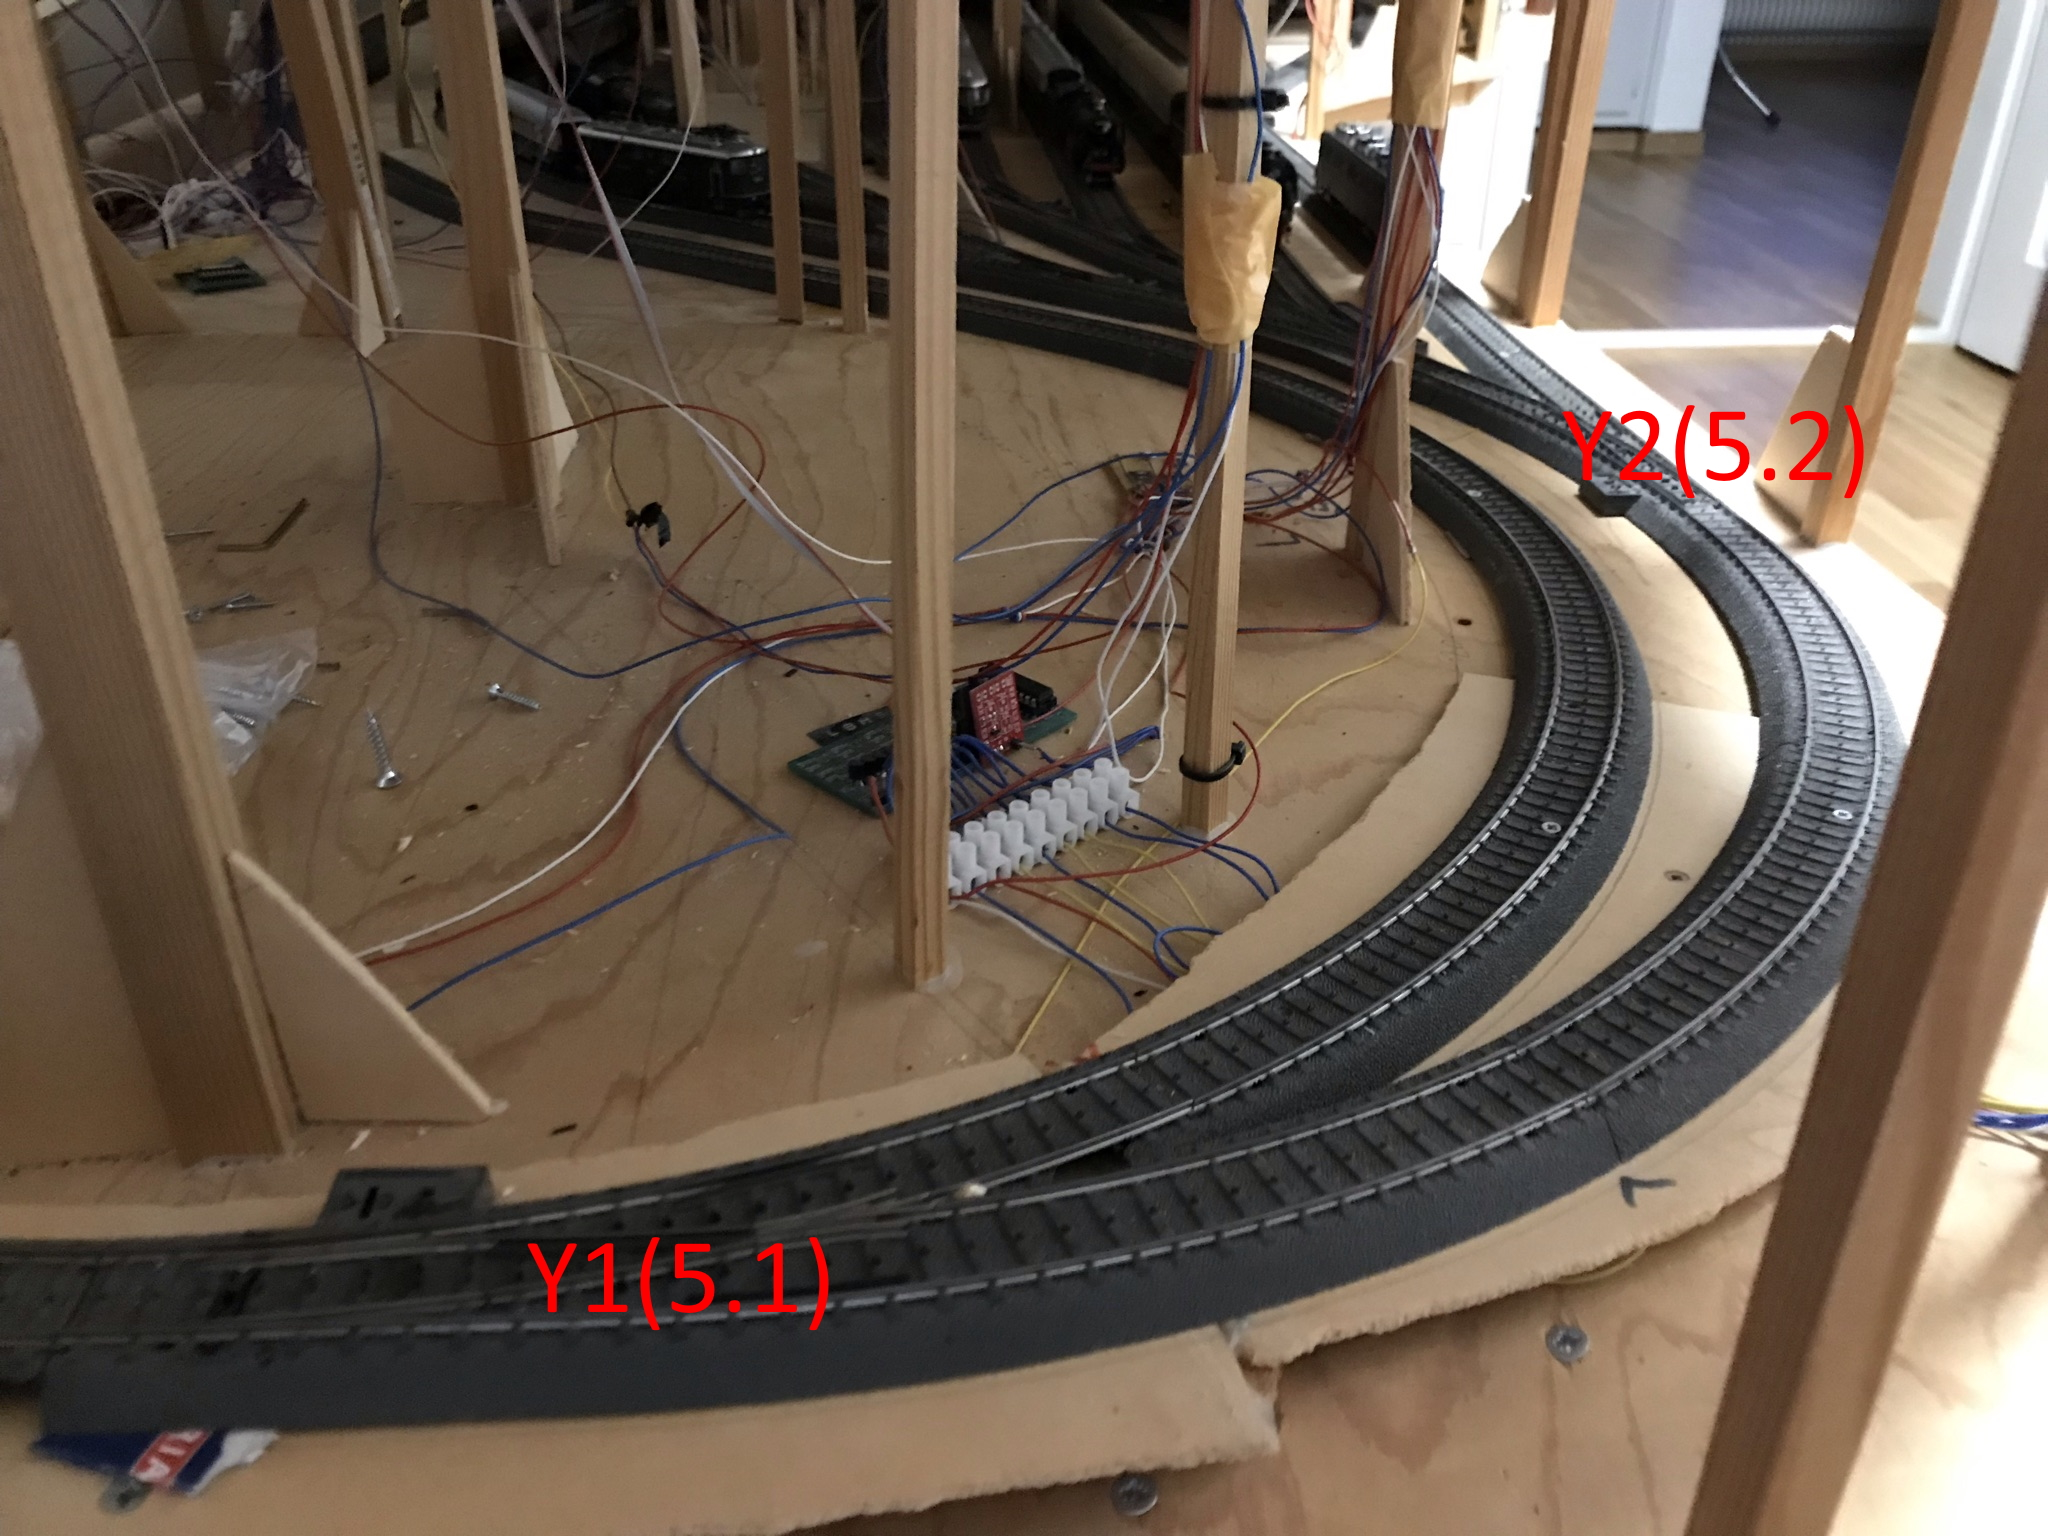
\includegraphics[width=0.75\textwidth]{ref/yard entry}
    \caption{Shadow Station: Entry Track}
\end{figure}
\begin{figure}[h!]
    \centering
    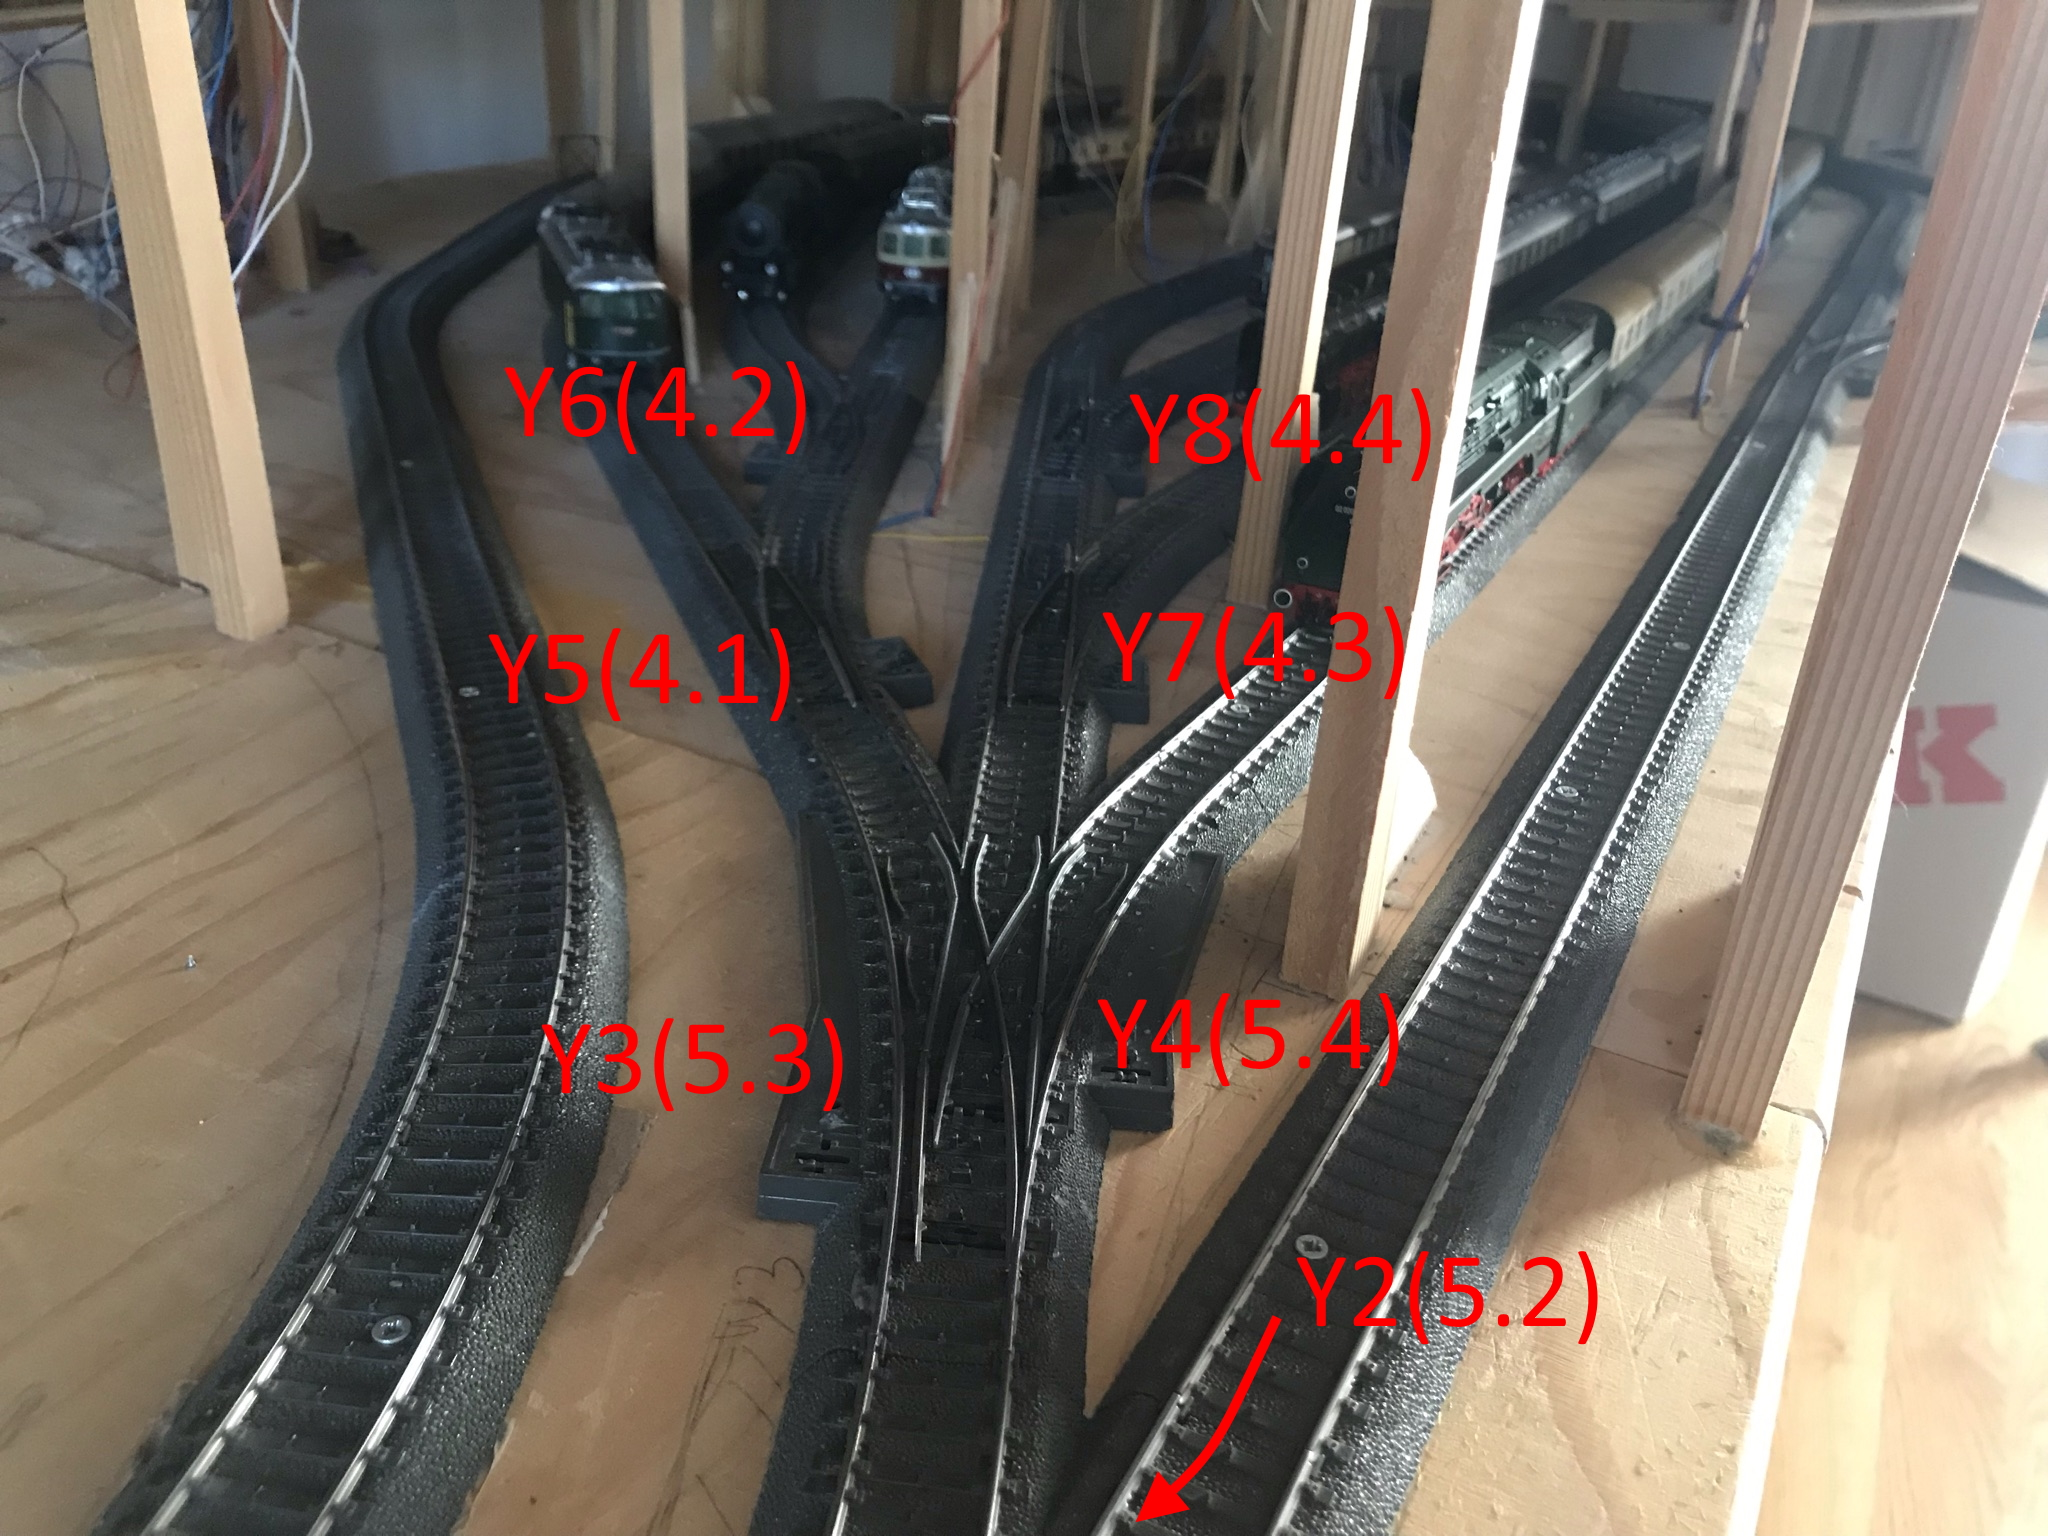
\includegraphics[width=0.8\textwidth]{ref/yard 2}
    \caption{Shadow Station: Primary Switching Area}
\end{figure}
\begin{figure}[h!]
    \centering
    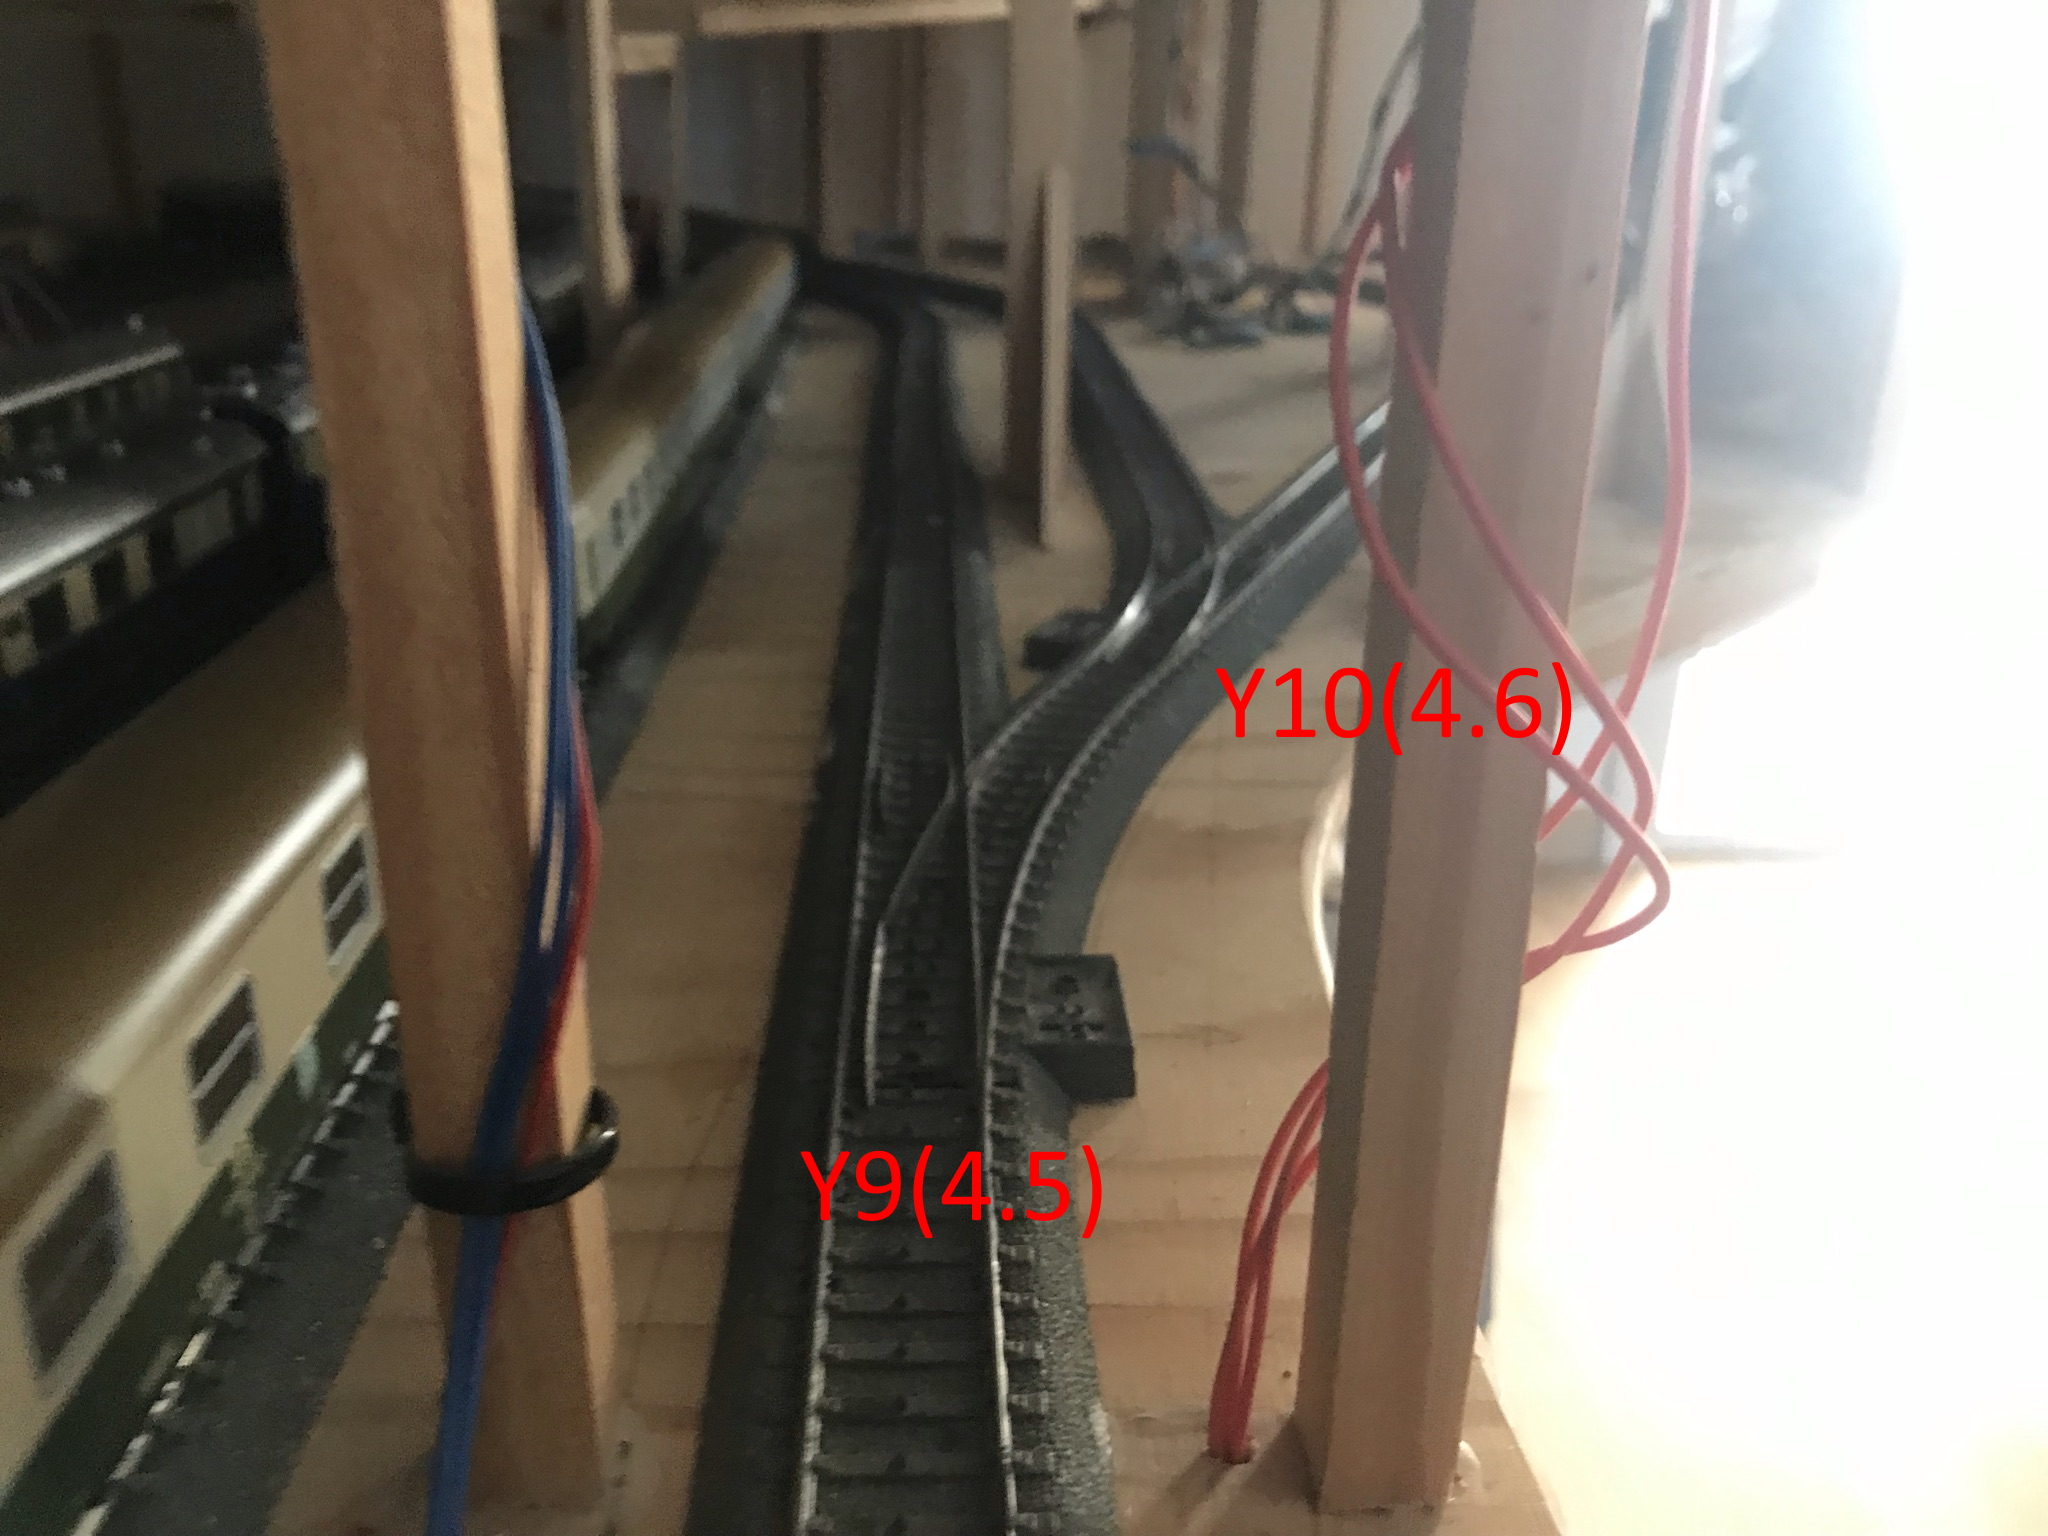
\includegraphics[width=0.8\textwidth]{ref/yard 3}
    \caption{Shadow Station: Auxilliary Switching Area}
\end{figure}
\begin{figure}[h!]
    \centering
    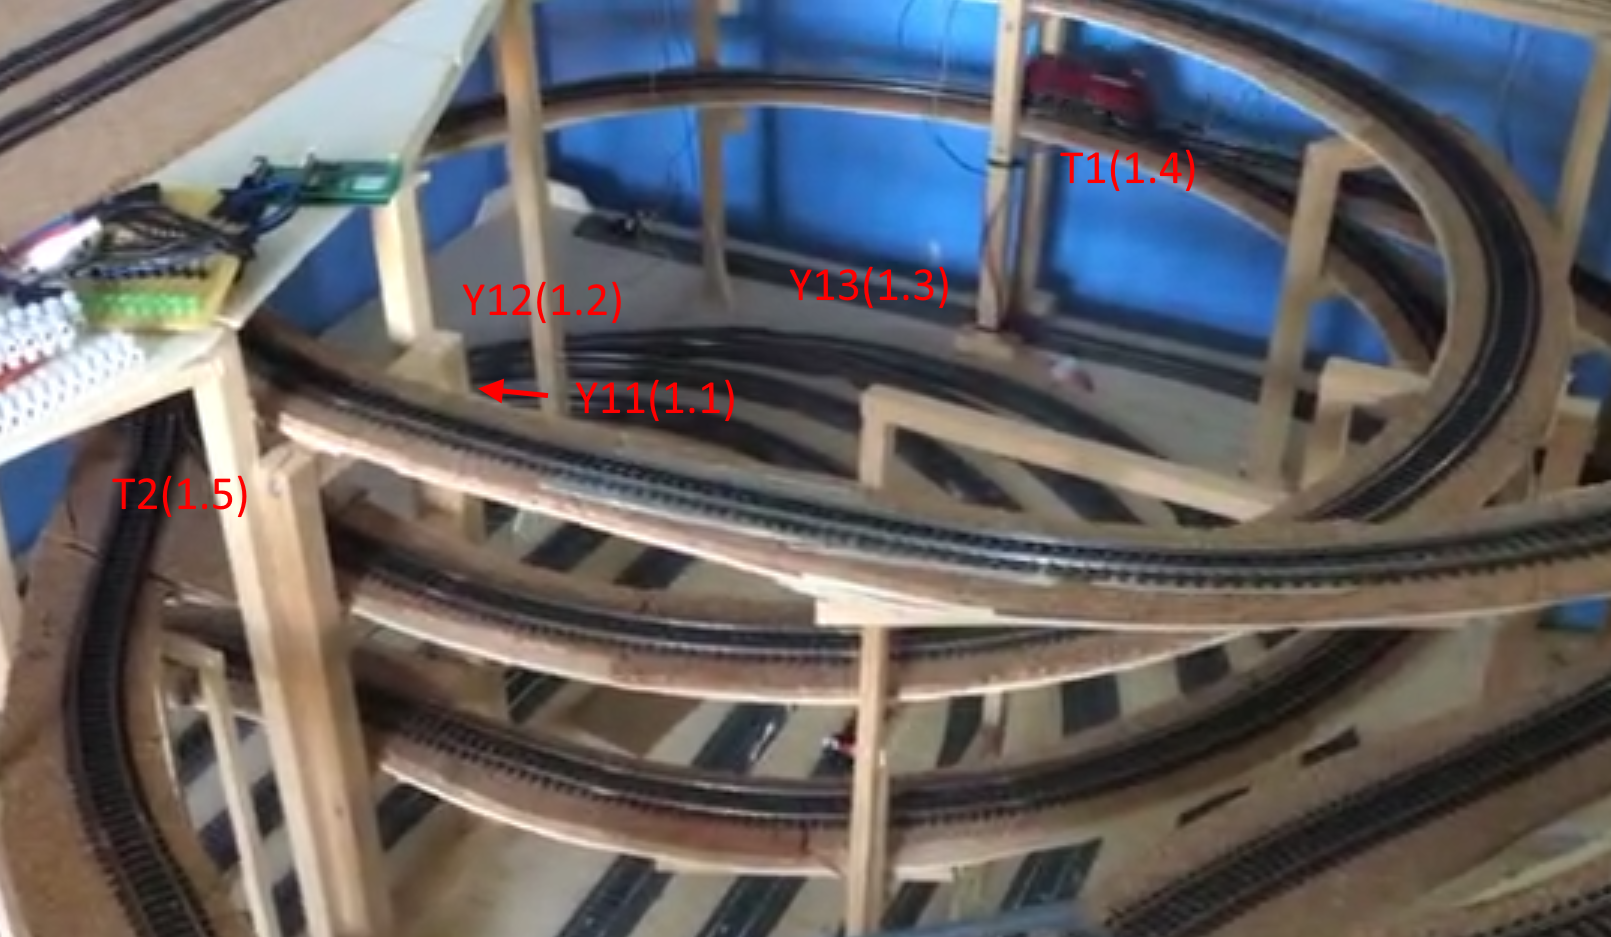
\includegraphics[width=0.8\textwidth]{ref/yard secondary exit and track spiral}
    \caption{Shadow Station: Secondary Station Exit (Y11-Y13)}
				Track Switches: Right Spiral (T1/T2)
\end{figure}
\begin{figure}[h!]
	\centering
	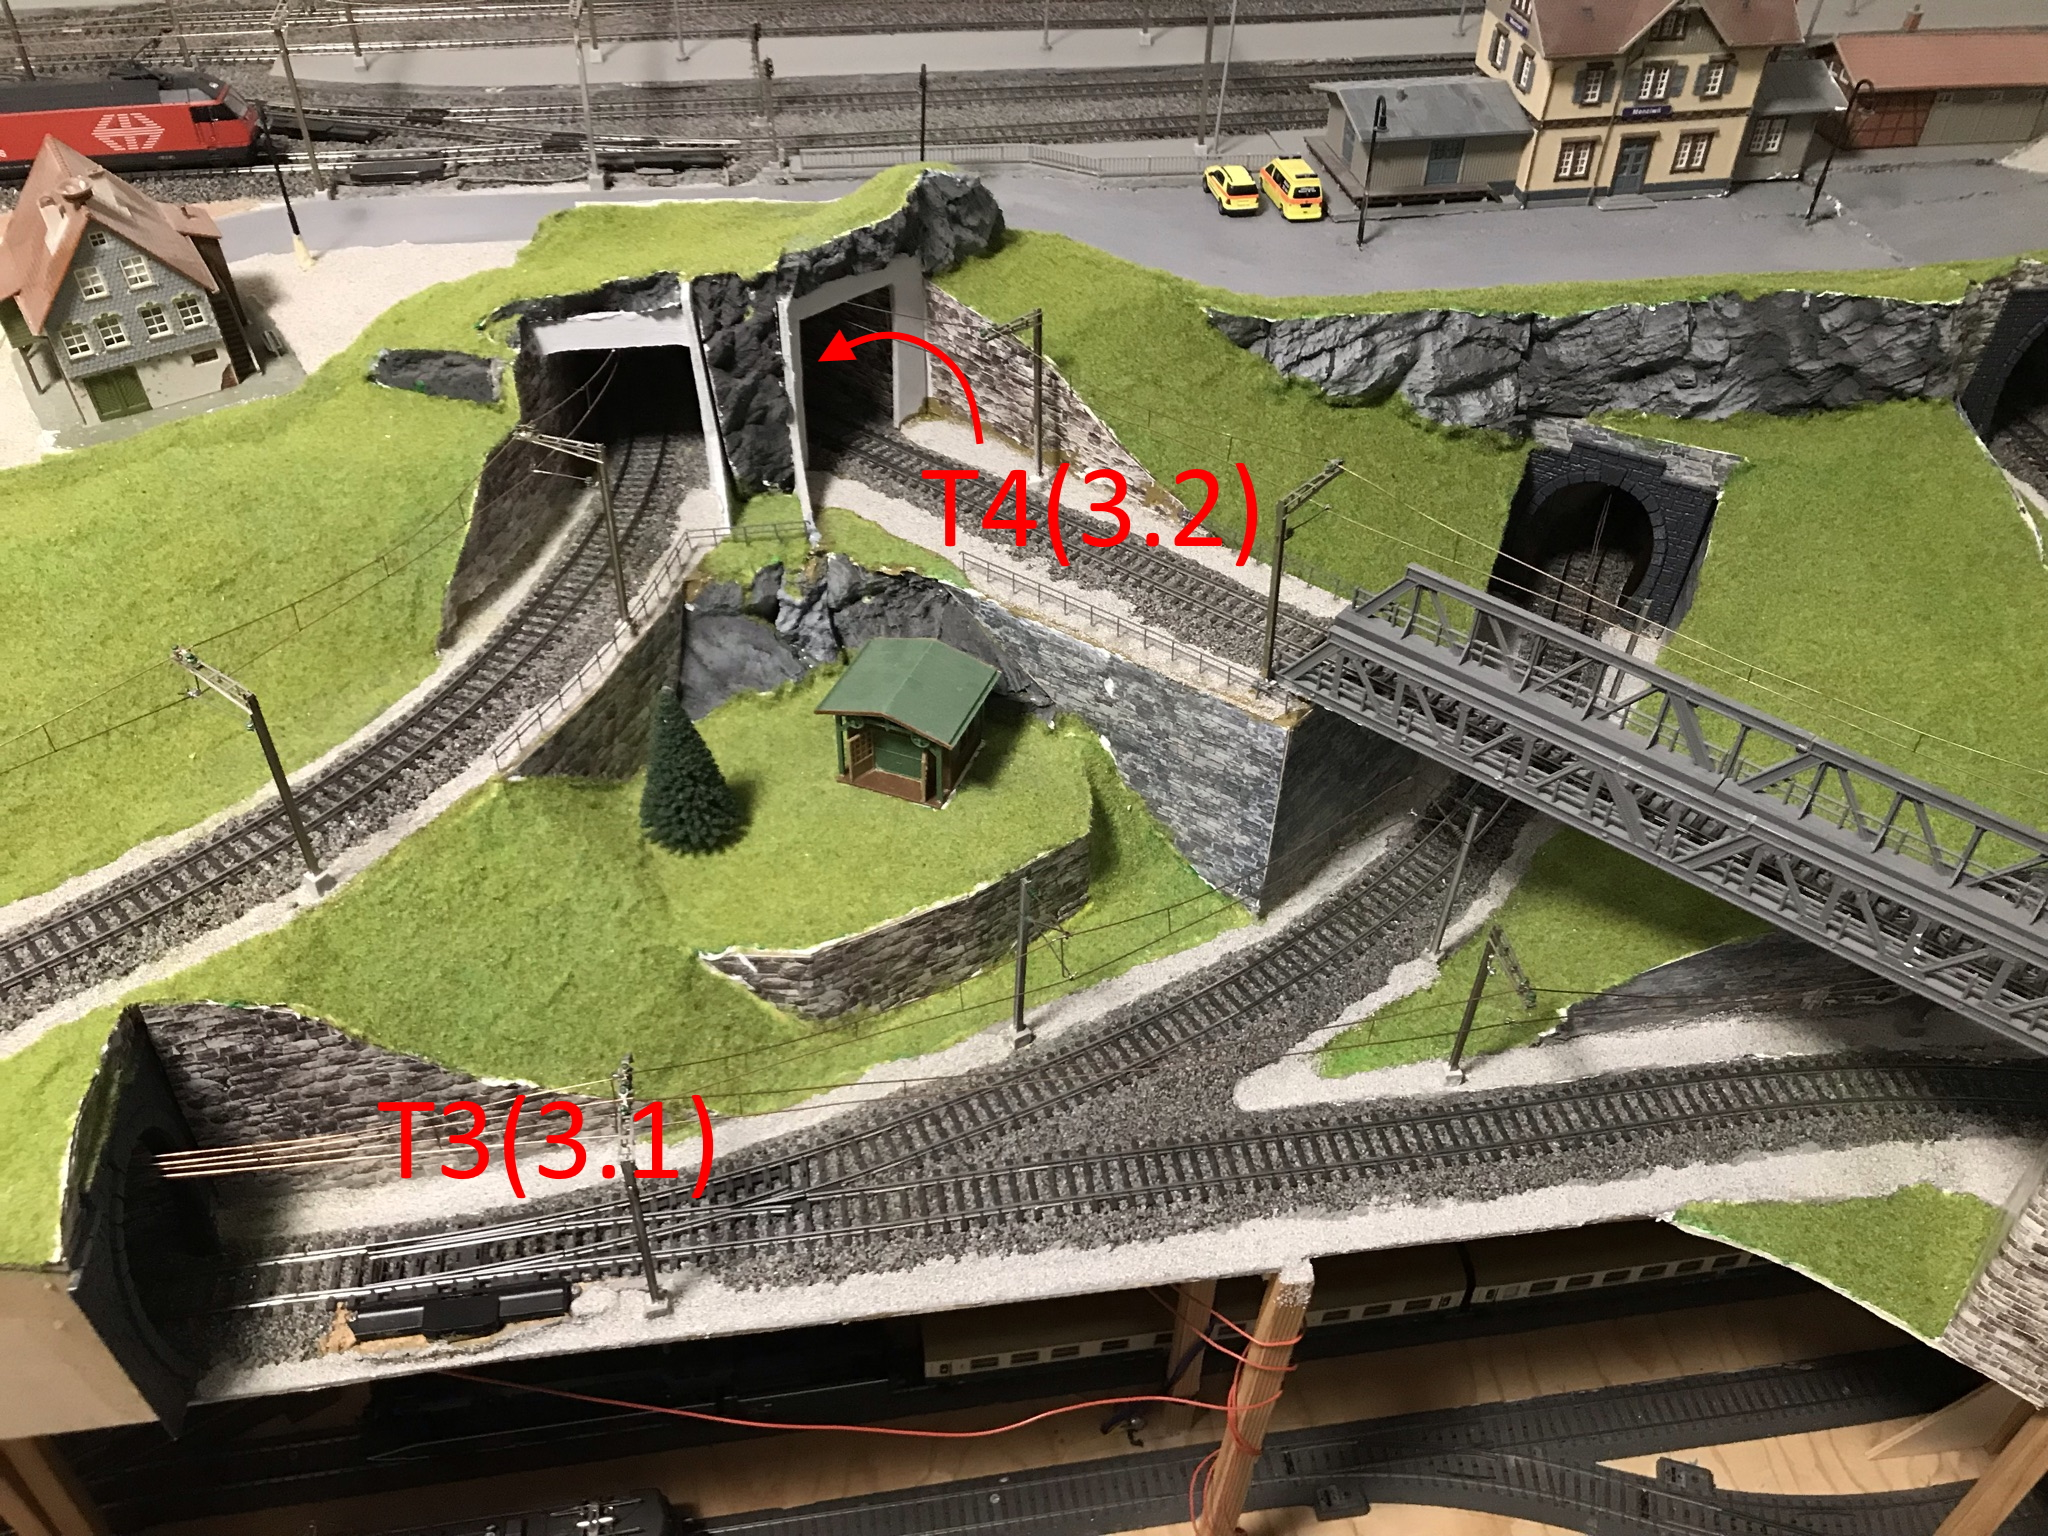
\includegraphics[width=0.8\textwidth]{ref/track top}
	\caption{Track Switches: Surface Switches}
\end{figure}
\begin{figure}[h!]
	\centering
	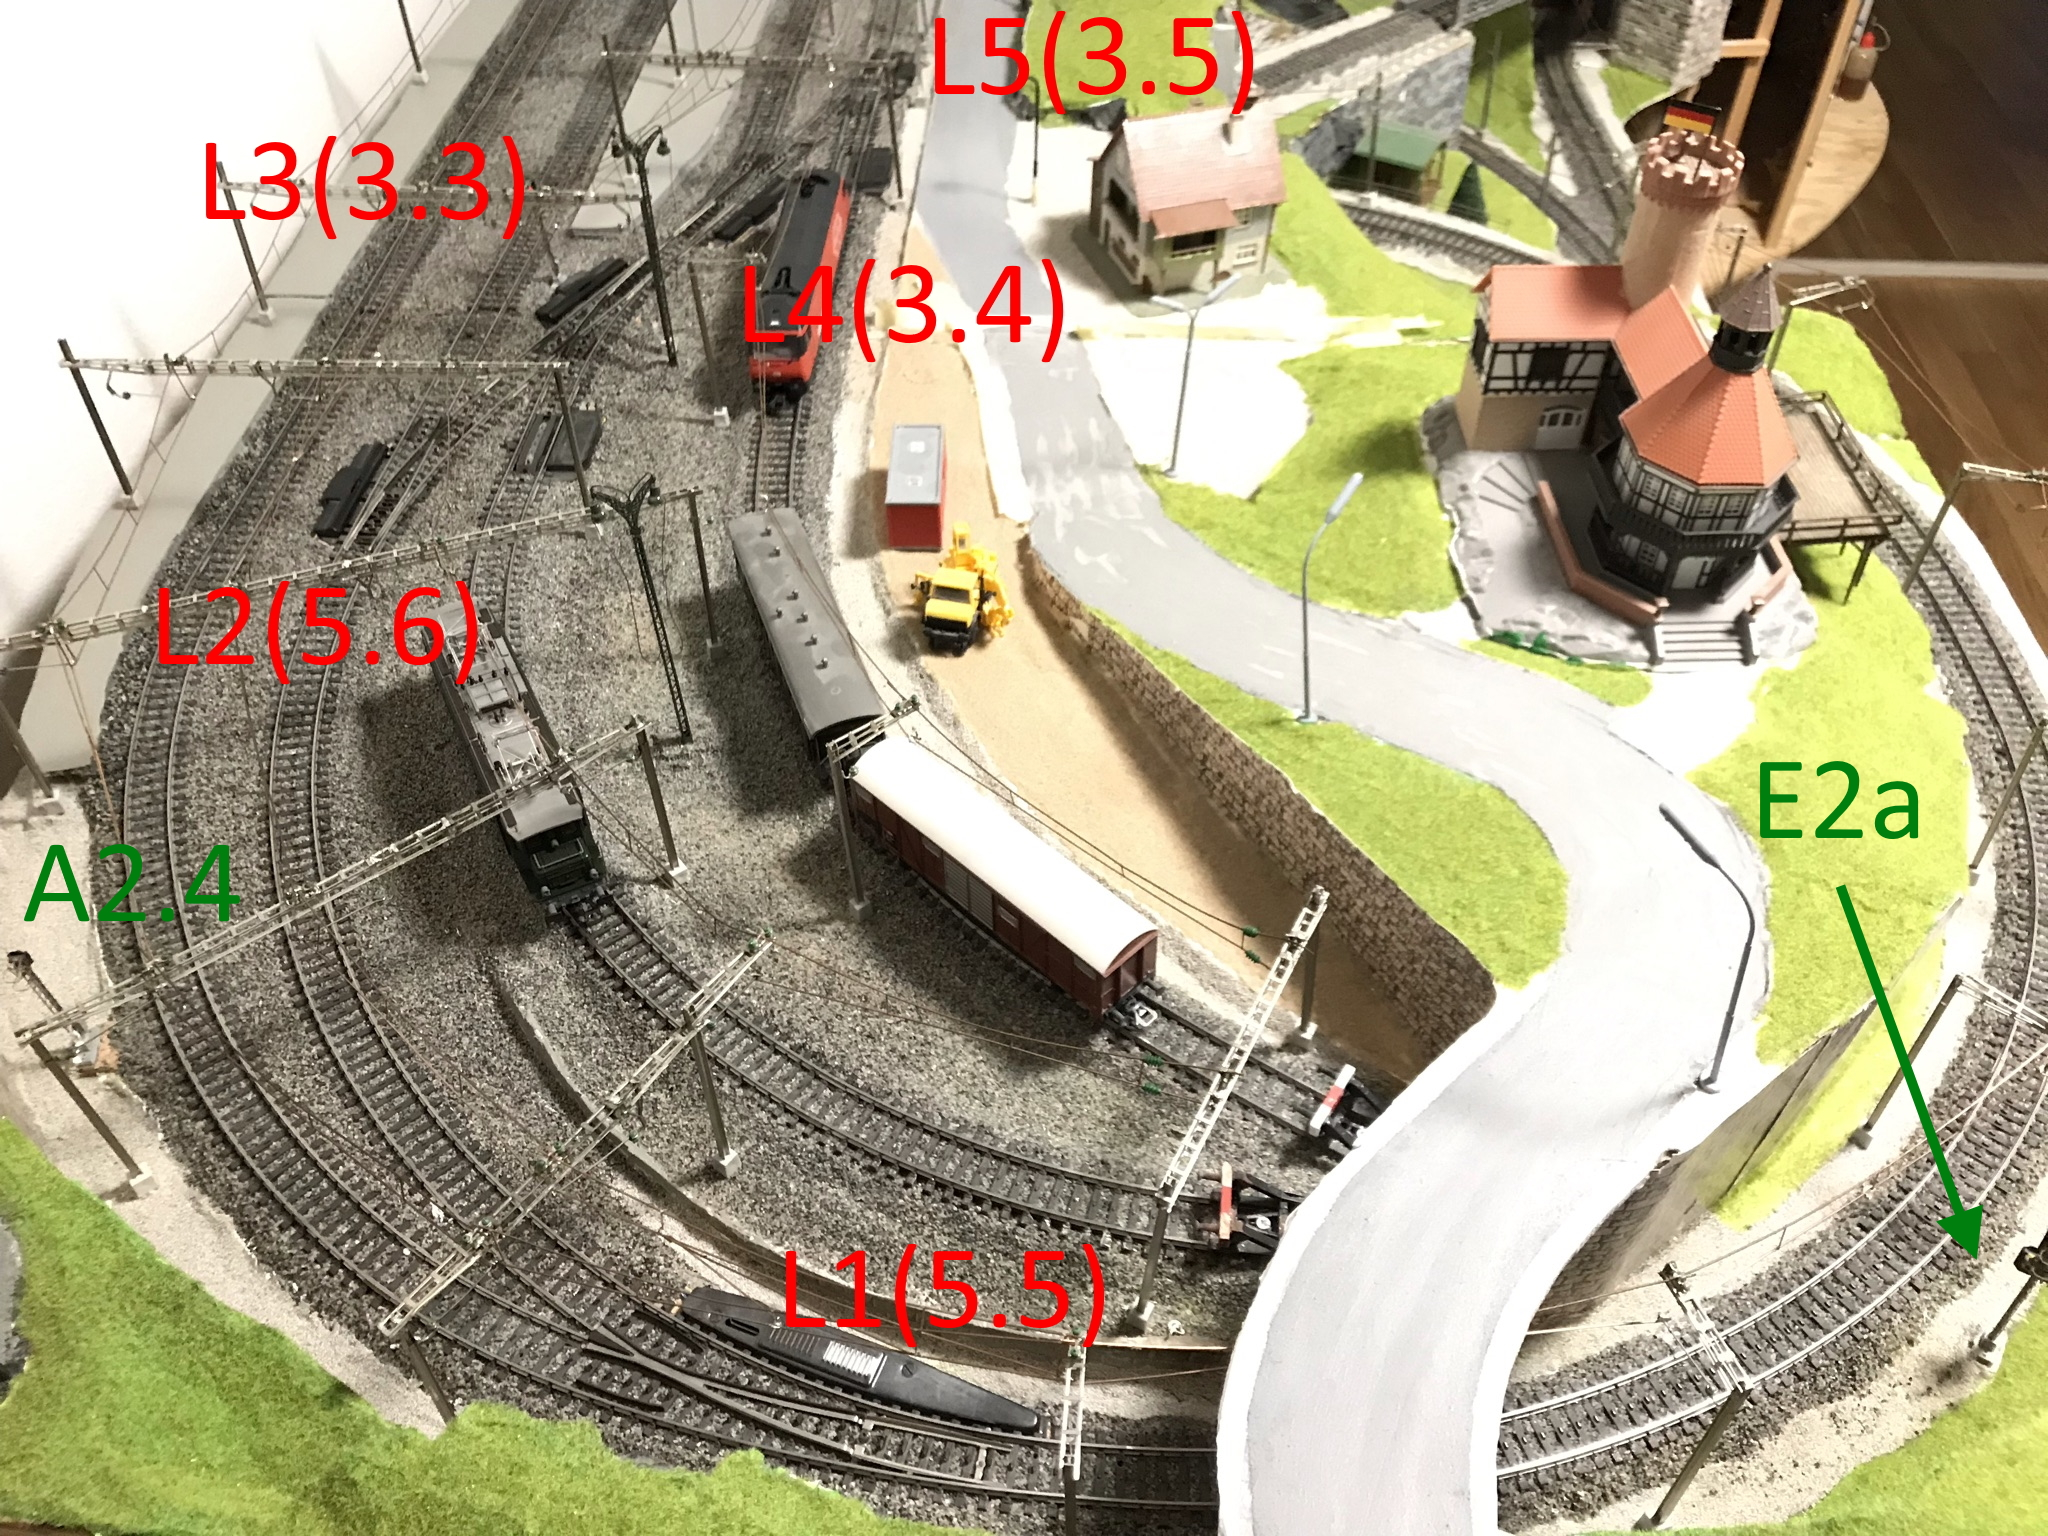
\includegraphics[width=0.8\textwidth]{ref/left overview}
	\caption{Station Entry Left: Overview}
\end{figure}
\begin{figure}[h!]
	\centering
	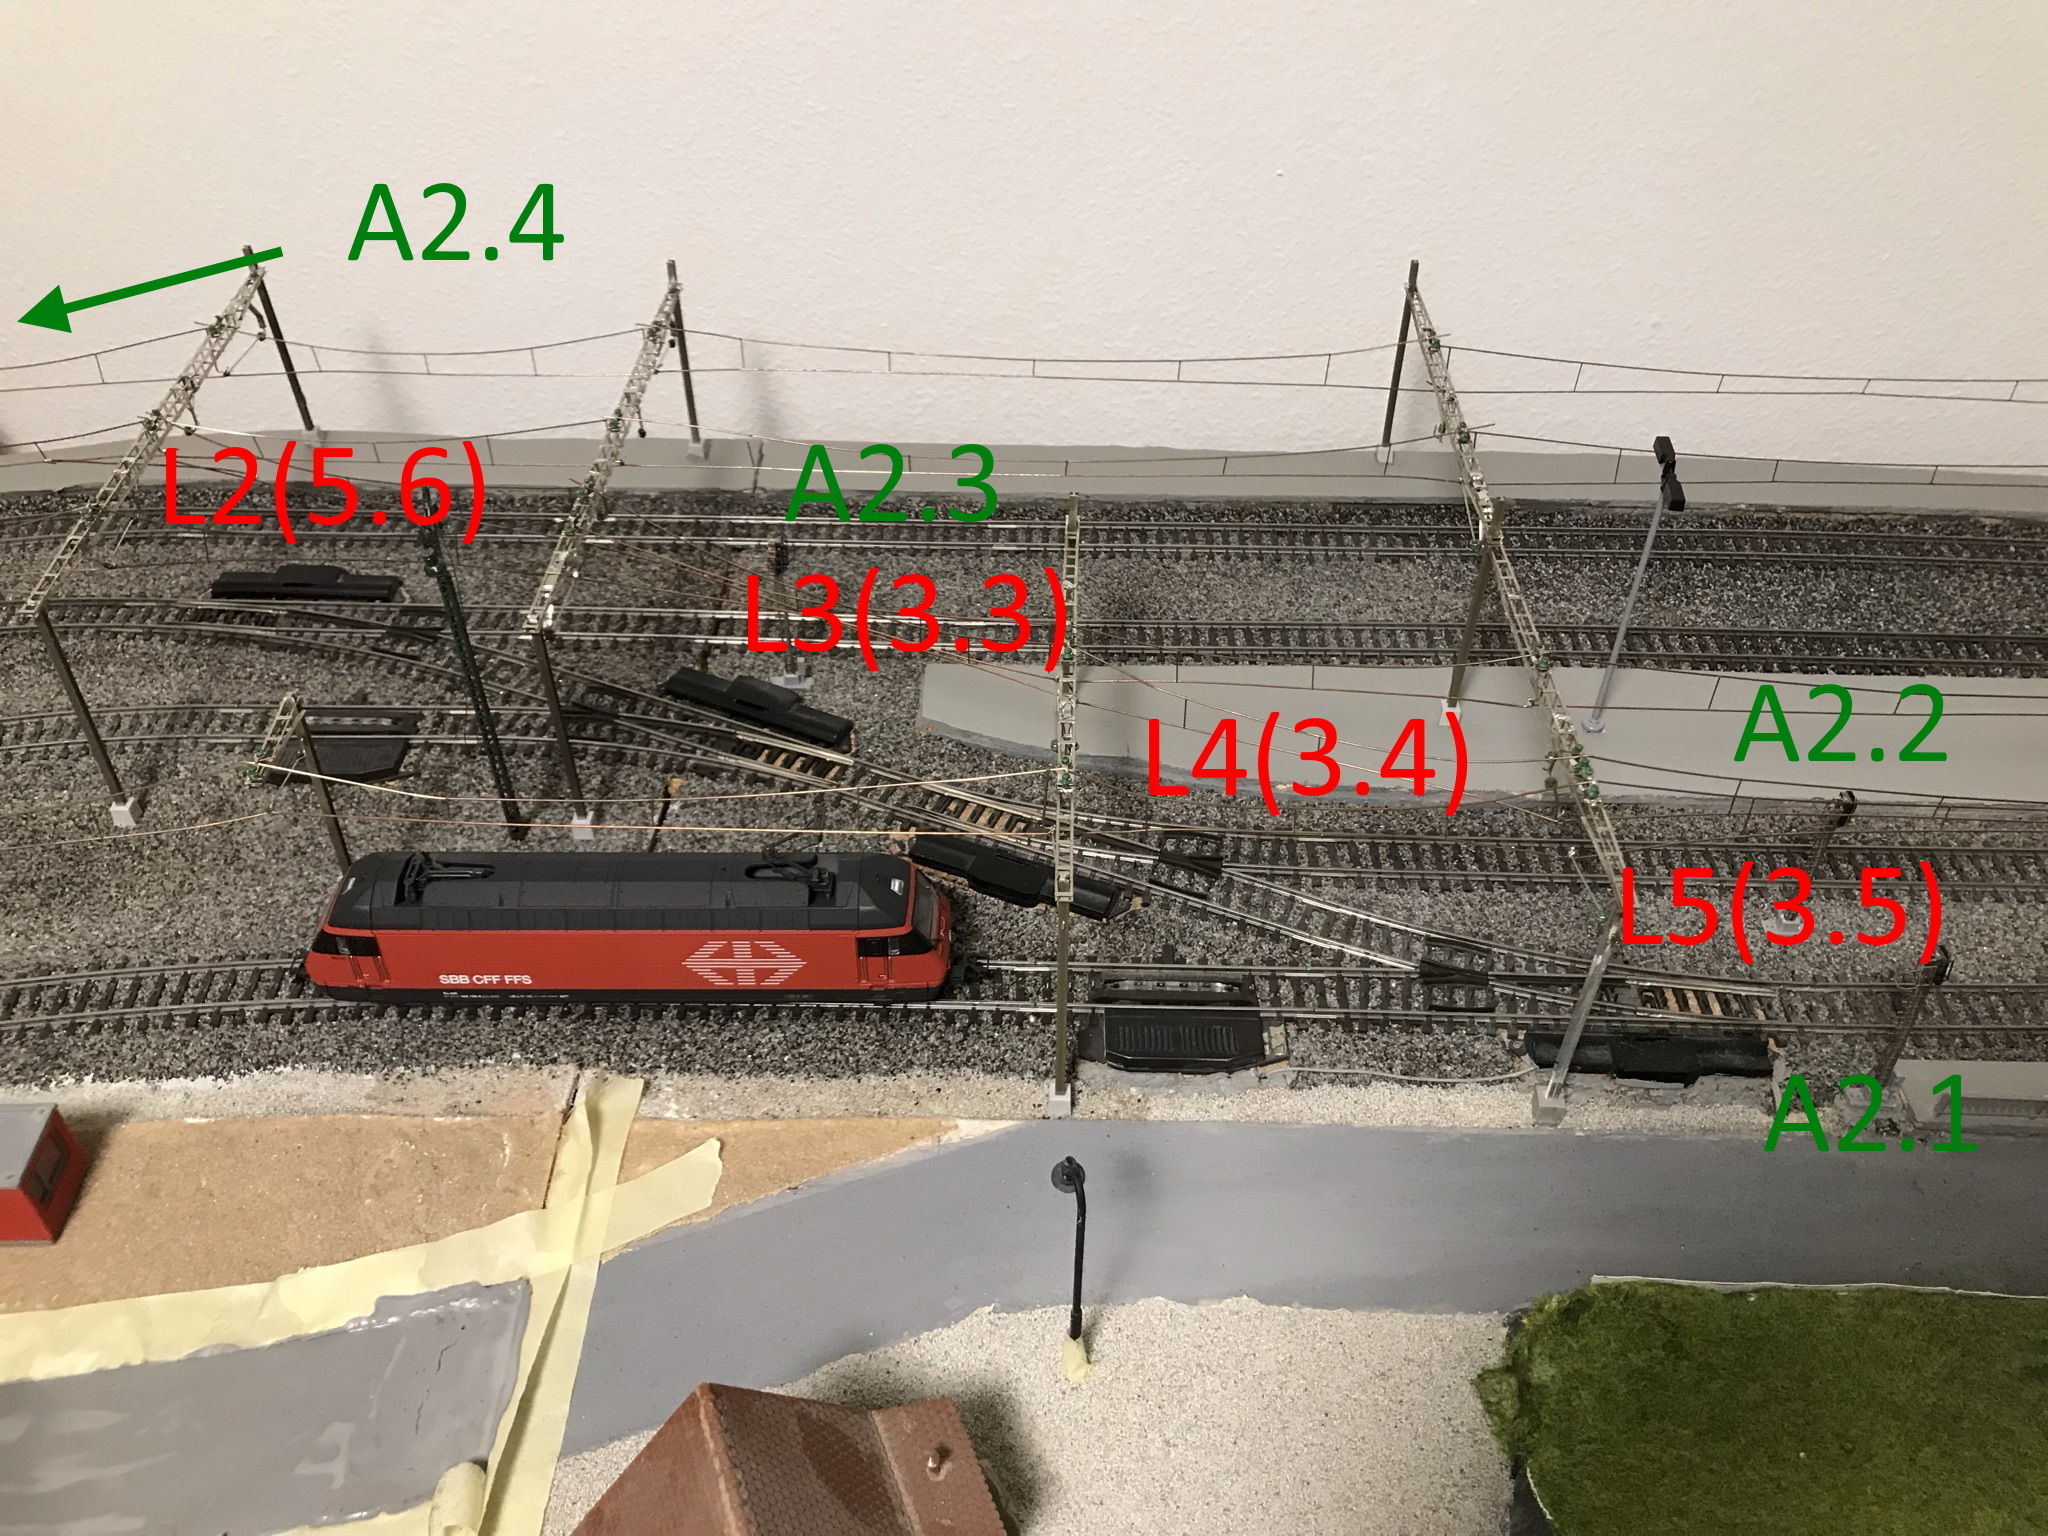
\includegraphics[width=0.8\textwidth]{ref/left details}
	\caption{Station Entry Left: Details View}
\end{figure}
\begin{figure}[h!]
	\centering
	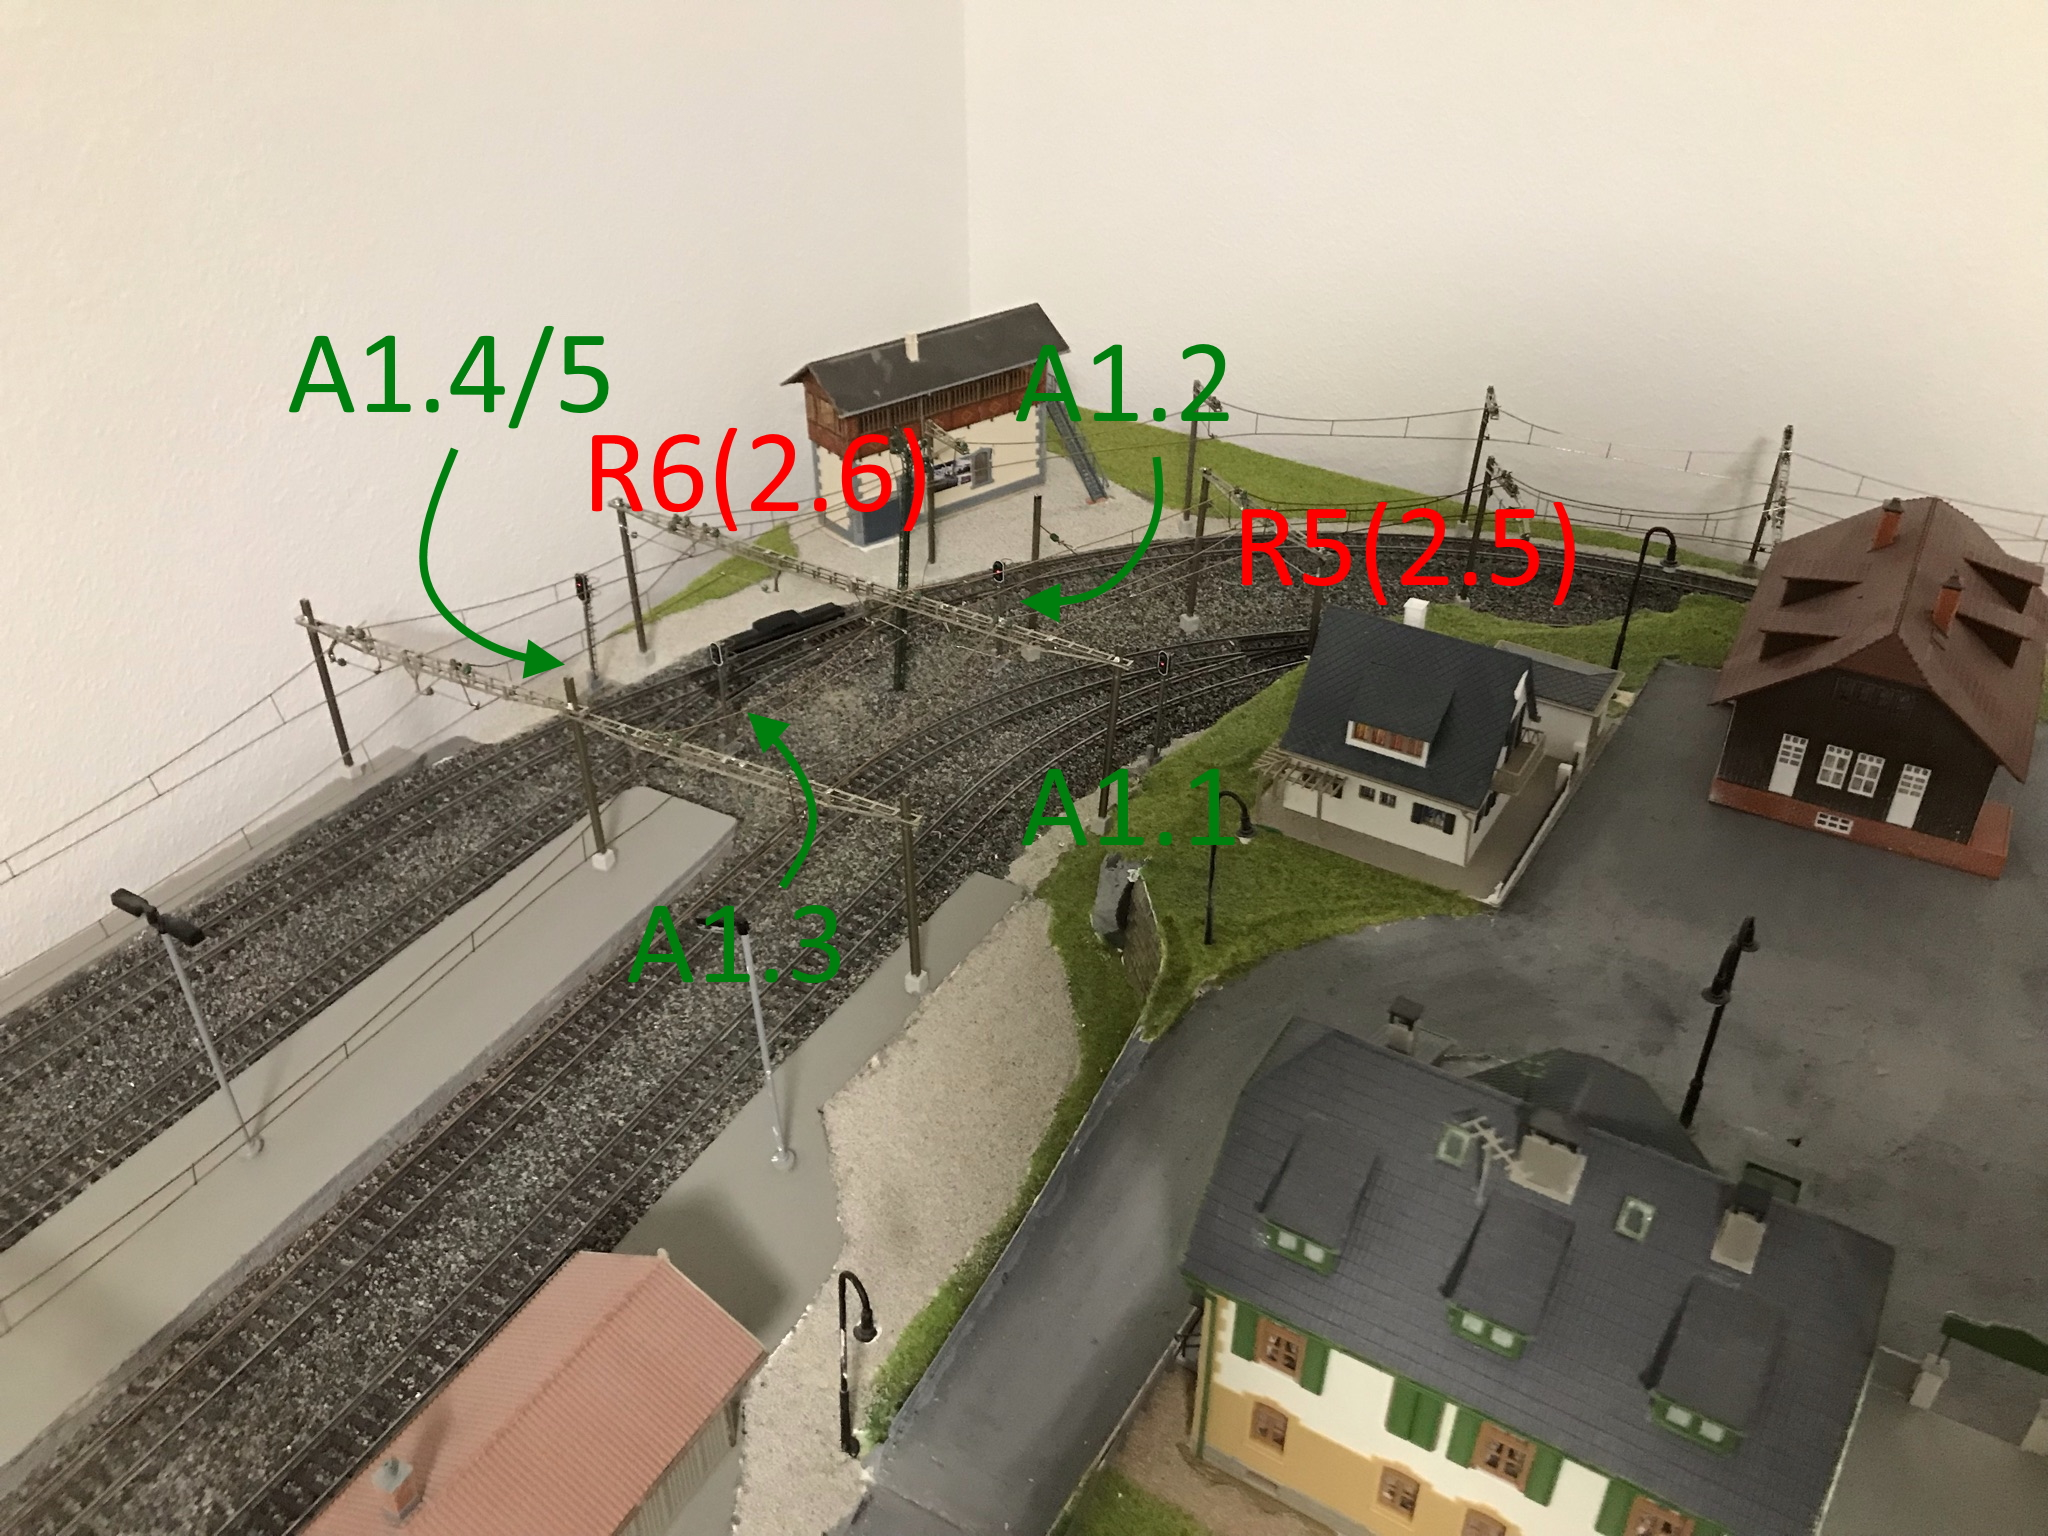
\includegraphics[width=0.8\textwidth]{ref/right rear}
	\caption{Station Entry Right: Rear View}
\end{figure}
\begin{figure}[h!]
	\centering
	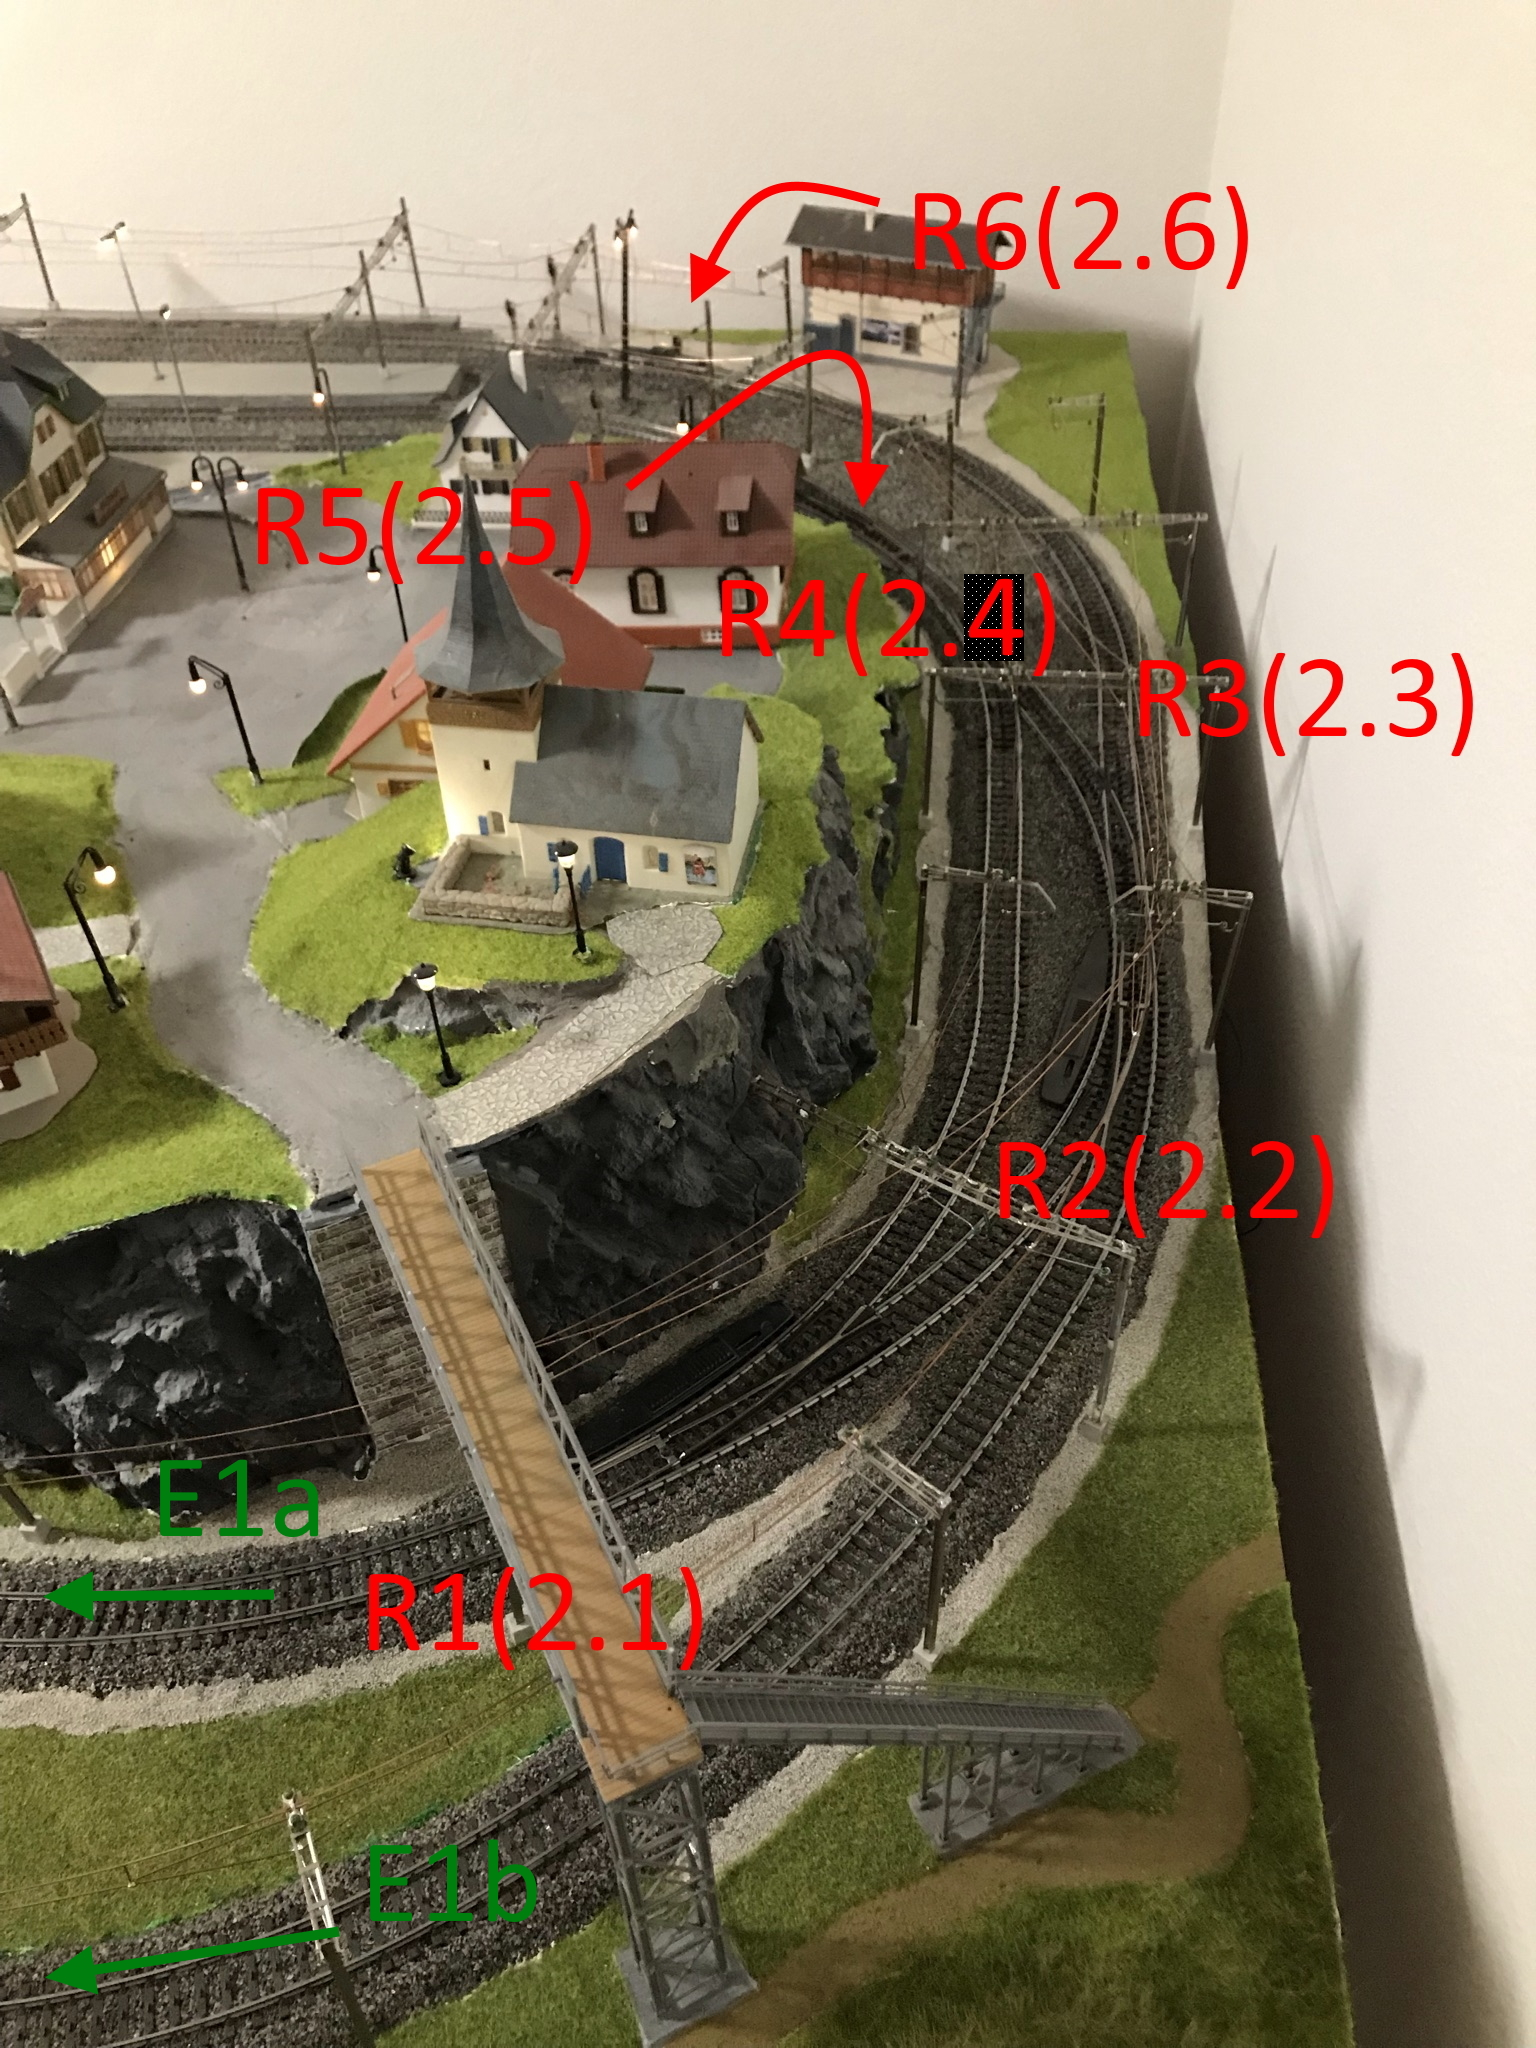
\includegraphics[width=0.8\textwidth]{ref/right front}
	\caption{Station Entry Right: Front View}
\end{figure}



\end{appendices}

\end{document}
